\documentclass[]{book}
\usepackage{lmodern}
\usepackage{amssymb,amsmath}
\usepackage{ifxetex,ifluatex}
\usepackage{fixltx2e} % provides \textsubscript
\ifnum 0\ifxetex 1\fi\ifluatex 1\fi=0 % if pdftex
  \usepackage[T1]{fontenc}
  \usepackage[utf8]{inputenc}
\else % if luatex or xelatex
  \ifxetex
    \usepackage{mathspec}
  \else
    \usepackage{fontspec}
  \fi
  \defaultfontfeatures{Ligatures=TeX,Scale=MatchLowercase}
\fi
% use upquote if available, for straight quotes in verbatim environments
\IfFileExists{upquote.sty}{\usepackage{upquote}}{}
% use microtype if available
\IfFileExists{microtype.sty}{%
\usepackage{microtype}
\UseMicrotypeSet[protrusion]{basicmath} % disable protrusion for tt fonts
}{}
\usepackage[margin=1in]{geometry}
\usepackage{hyperref}
\hypersetup{unicode=true,
            pdftitle={L'inférence Statistique},
            pdfauthor={Jean-Marc Meunier},
            pdfborder={0 0 0},
            breaklinks=true}
\urlstyle{same}  % don't use monospace font for urls
\usepackage{natbib}
\bibliographystyle{apalike}
\usepackage{longtable,booktabs}
\usepackage{graphicx,grffile}
\makeatletter
\def\maxwidth{\ifdim\Gin@nat@width>\linewidth\linewidth\else\Gin@nat@width\fi}
\def\maxheight{\ifdim\Gin@nat@height>\textheight\textheight\else\Gin@nat@height\fi}
\makeatother
% Scale images if necessary, so that they will not overflow the page
% margins by default, and it is still possible to overwrite the defaults
% using explicit options in \includegraphics[width, height, ...]{}
\setkeys{Gin}{width=\maxwidth,height=\maxheight,keepaspectratio}
\IfFileExists{parskip.sty}{%
\usepackage{parskip}
}{% else
\setlength{\parindent}{0pt}
\setlength{\parskip}{6pt plus 2pt minus 1pt}
}
\setlength{\emergencystretch}{3em}  % prevent overfull lines
\providecommand{\tightlist}{%
  \setlength{\itemsep}{0pt}\setlength{\parskip}{0pt}}
\setcounter{secnumdepth}{5}
% Redefines (sub)paragraphs to behave more like sections
\ifx\paragraph\undefined\else
\let\oldparagraph\paragraph
\renewcommand{\paragraph}[1]{\oldparagraph{#1}\mbox{}}
\fi
\ifx\subparagraph\undefined\else
\let\oldsubparagraph\subparagraph
\renewcommand{\subparagraph}[1]{\oldsubparagraph{#1}\mbox{}}
\fi

%%% Use protect on footnotes to avoid problems with footnotes in titles
\let\rmarkdownfootnote\footnote%
\def\footnote{\protect\rmarkdownfootnote}

%%% Change title format to be more compact
\usepackage{titling}

% Create subtitle command for use in maketitle
\newcommand{\subtitle}[1]{
  \posttitle{
    \begin{center}\large#1\end{center}
    }
}

\setlength{\droptitle}{-2em}
  \title{L'inférence Statistique}
  \pretitle{\vspace{\droptitle}\centering\huge}
  \posttitle{\par}
  \author{Jean-Marc Meunier}
  \preauthor{\centering\large\emph}
  \postauthor{\par}
  \predate{\centering\large\emph}
  \postdate{\par}
  \date{2018-05-11}

\usepackage{booktabs}

\usepackage{amsthm}
\newtheorem{theorem}{Theorem}[chapter]
\newtheorem{lemma}{Lemma}[chapter]
\theoremstyle{definition}
\newtheorem{definition}{Definition}[chapter]
\newtheorem{corollary}{Corollary}[chapter]
\newtheorem{proposition}{Proposition}[chapter]
\theoremstyle{definition}
\newtheorem{example}{Example}[chapter]
\theoremstyle{definition}
\newtheorem{exercise}{Exercise}[chapter]
\theoremstyle{remark}
\newtheorem*{remark}{Remark}
\newtheorem*{solution}{Solution}
\begin{document}
\maketitle

{
\setcounter{tocdepth}{1}
\tableofcontents
}
\hypertarget{introduction}{%
\chapter*{INTRODUCTION}\label{introduction}}
\addcontentsline{toc}{chapter}{INTRODUCTION}

Ce document constitue la version enrichi du support de cours des
étudiants de licence de pyschologie à l'institut d'enseignement à
distance de l'Université Paris 8. L'enrichissement du cours a été
réalisé dans le cadre du projet Ontostat, financé par le ministère de
l'enseignement supérieur, de la recherche et de l'innovation français
dans le cadre de l'appel à manifestation d'intérêt de la mission pour
innovation et la pédagogie numérique dans l'enseignement supérieur
(MIPNES). Il constitue un prototype viusant à instrumentaliser une
ontologie des concepts statistiques développée par l'université d'Oxford
(Stato).

\hypertarget{presentation-du-cours}{%
\section*{Présentation du cours}\label{presentation-du-cours}}
\addcontentsline{toc}{section}{Présentation du cours}

En première année, vous avez eu à étudier les méthodes descriptives
d'analyse de données. Ces méthodes sont applicables à différents types
d'objets : variable, protocole et distribution. Elles visent pour
l'essentiel à résumer les données et à tirer un certain nombre de
conclusions sur l'échantillon observé. La portée de ces conclusions ne
peut cependant pas dépasser l'échantillon, c'est pourquoi ces méthodes
sont dites descriptives. Avec les méthodes inférentielles, qui seront
abordées dans ce cours, nous allons voir sous quelles conditions les
conclusions descriptives peuvent être étendues à la population d'où est
issue l'échantillon. L'idée de base qui préside à l'inférence
statistique est que l'échantillon observé est un des échantillons
possibles. Partant de là, la démarche consiste à situer l'échantillon
observé dans cet ensemble d'échantillons possibles. Il s'agit en fait
d'une généralisation aux protocoles de la méthode permettant de situer
un individu dans une distribution (voir le cours de licence première
année)

La démarche générale reste la même quel que soit le type de protocole.
Cependant la méthodologie varie en fonction (i) de l'échelle de mesure
de la variable observée (ii) mais surtout de la structuration du
protocole. C'est pour cette raison que ce cours est structuré en
fonction des types de protocoles sur lesquels porte l'inférence. Nous
aurions pu, à l'instar, de certains manuels, structurer ce cours en
distinguant les tests paramétriques et les tests non paramétriques. Une
structuration du cours fondée sur les propriétés des protocoles nous
paraît cependant préférable à une structuration fondée sur la nature du
test pour trois raisons. D'abord une telle structuration permet de
mettre en évidence les similitudes dans les démarches d'analyses des
protocoles nominaux et des protocoles numériques et nous verrons à
travers l'inférence combinatoire que ces similitudes sont tout à fait
importantes. Ensuite, une telle structuration permet de montrer comment
la démarche inférentielle sur un protocole non structuré peut être
généralisée à des protocoles structurés. Enfin, et c'est à nos yeux
l'argument le plus important, au moment de choisir le type de test à
appliquer, que ce soit dans le cadre d'une recherche ou plus simplement
le jour de l'examen, ce sont les propriétés du protocole qui sont les
plus disponibles et qui doivent guider le chercheur dans sa démarche
d'analyse et non les propriétés du test.

Ce cours, complété par les séquences audiovisuelles disponibles sur
notre plate-forme d'enseignement à distance, est donc structuré en cinq
chapitres. Le premier chapitre est consacré aux principes généraux de
l'inférence et à la définition des principaux concepts. Dans le deuxième
chapitre, nous aborderons l'inférence sur les protocoles univariés non
structurés. Nous verrons ensuite l'inférence sur les protocoles
structurés par un croisement, dans le chapitre 3, et par un emboîtement,
dans le chapitre 4. Enfin, dans le dernier chapitre, nous aborderons
l'inférence sur les protocoles bivariés.

\hypertarget{principes-et-methodologie}{%
\chapter{PRINCIPES ET METHODOLOGIE}\label{principes-et-methodologie}}

\hypertarget{definition-des-principaux-concepts}{%
\section{Définition des principaux
concepts}\label{definition-des-principaux-concepts}}

L'inférence statistique utilise un certain nombre de concepts qu'il
convient de connaître et pour certains de ne pas confondre. Nous allons
donc dans un premier temps poser les définitions de ces concepts. Les
analyses statistiques, quelles qu'elles soient, portent sur un protocole
recueilli sur un échantillon issu d'une population parente.

\begin{itemize}
\tightlist
\item
  \textbf{Protocole}. Ensemble d'observations sur une ou plusieurs
  variables.
\item
  \textbf{Échantillon}. Ensemble d'individus statistiques sur lesquels
  sont recueillies les données constituant le protocole. L'échantillon
  est un sous-ensemble de la population.
\item
  \textbf{Population parente}. Également appelée population, c'est
  l'ensemble des individus statistiques d'où est extrait l'échantillon.
  La population parente est de taille finie. On distinguera
  l'échantillonnage dans une population et l'échantillonnage dans une
  distribution.
\item
  \textbf{Échantillonnage dans une population}. C'est l'extraction d'un
  échantillon dans ensemble de référence de taille finie.
  L'échantillonnage dans une population peut être vu comme un tirage
  sans remise.
\item
  \textbf{Échantillonnage dans une distribution}. C'est l'extraction
  d'un échantillon dans un ensemble de référence de taille infinie.
  Cette forme d'échantillonnage peut être assimilée à un tirage avec
  remise dans une population finie.
\end{itemize}

Le principe général de l'inférence consiste à situer un échantillon dans
l'espace des échantillons. Pour cela, on situe un résumé du protocole
dans une distribution d'échantillonnage. La conclusion de cette
inférence dépend du modèle d'échantillonnage choisi.

\begin{itemize}
\tightlist
\item
  \textbf{Espace des échantillons}. C'est l'ensemble de tous les
  échantillons possibles obtenus par combinatoire.
\item
  \textbf{Distribution d'échantillonnage}. C'est la distribution, pour
  une statistique donnée, de l'ensemble des échantillons possibles. Pour
  les variables numériques, la distribution d'échantillonnage est faite
  sur la moyenne. Pour les variables nominales ou catégorisées, on
  utilise généralement la fréquence pour construire la distribution
  d'échantillonnage.
\item
  \textbf{Modèle d'échantillonnage}. C'est l'ensemble des hypothèses que
  l'on fait sur le mode de constitution de l'échantillon à partir de la
  population.
\end{itemize}

\hypertarget{principes-generaux-de-linference}{%
\section{Principes généraux de
l'inférence}\label{principes-generaux-de-linference}}

L'inférence statistique est une forme de raisonnement
hypothético-déductif. Dans cette forme de raisonnement, on cherche à
tester une hypothèse à travers un raisonnement déductif dont la démarche
suit le questionnement suivant :

\begin{itemize}
\tightlist
\item
  Dans un premier temps, la démarche consiste à se demander quel est
  l'ensemble des protocoles possibles. Cet ensemble de protocoles est
  obtenu par combinatoire, d'où le nom de cette approche, Dans cette
  approche, le protocole observé est un des protocoles possibles, mais
  n'est pas nécessairement tiré au hasard.
\item
  Ensuite on cherche à situer le protocole observé dans l'ensemble des
  protocoles possibles. Pour cela, on calcule sur chacun des protocoles
  possibles une statistique résumant les protocoles (statistique
  d'échantillonnage). Dans le cas des variables catégorisées,
  c'est-à-dire nominale ou ordinale, cette statistique est la fréquence.
  Dans le cas des variables numériques, cette statistique est la
  moyenne. Ces statistiques résumant les protocoles sont utilisées pour
  calculer une distribution qui permettra de situer le protocole observé
  dans l'ensemble des protocoles possibles. Cette distribution est ce
  qu'on appelle distribution d'échantillonnage.
\item
  Enfin, on se demandera si le protocole observé est suffisamment rare
  dans la distribution d'échantillonnage pour le considérer comme
  atypique ou si on doit le considérer comme typique.
\end{itemize}

\hypertarget{choix-du-modele-dechantillonnage}{%
\section{Choix du modèle
d'échantillonnage}\label{choix-du-modele-dechantillonnage}}

Le modèle d'échantillonnage est l'ensemble des hypothèses que l'on fait
sur le mode de constitution de l'échantillon à partir de la population.
Concrètement, le choix du modèle d'échantillonnage n'engage en rien le
choix de la distribution d'échantillonnage et de la procédure à mettre
en oeuvre. En revanche, le choix du modèle d'échantillonnage détermine
la formulation de la conclusion.

Dans tous les cas, on peut se placer dans le cadre du modèle
combinatoire qui consiste à considérer le protocole observé comme un
élément de l'ensemble des protocoles possibles (espace des
échantillons). La conclusion se formulera en termes de typicité
(comparaison d'un groupe d'observations à une distribution de référence)
ou d'homogénéité (comparaison de deux groupes d'observations).

On peut parfois se situer dans le cadre du modèle fréquentiste qui
consiste à considérer que la distribution d'échantillonnage est une
distribution des probabilités d'obtenir un échantillon de telle ou telle
moyenne. Ce modèle constitue un prolongement du modèle combinatoire.
Pour cela, on fait l'hypothèse supplémentaire que l'échantillon a été
tiré au hasard dans l'ensemble des protocoles possibles. Cette hypothèse
n'est justifiée que si la procédure expérimentale fait intervenir le
hasard (sondage ou aléatorisation de la répartition des sujets) ou si
l'expérience vise véritablement à tester une hypothèse, autrement dit
que la comparaison est faite toutes choses égales par ailleurs.

\hypertarget{choix-de-la-distribution-dechantillonnage}{%
\section{Choix de la distribution
d'échantillonnage}\label{choix-de-la-distribution-dechantillonnage}}

Ce choix dépend de l'échelle de mesure de la variable dépendante. On
distinguera les variables numériques, pour lesquelles on peut utiliser
des tests dits paramétriques des autres variables pour lesquelles on
utilise des tests non paramétriques.

Dans les deux cas, on peut utiliser une distribution exacte ou une
distribution approchée. Les distributions d'échantillonnage exactes sont
obtenues par combinatoire ou en ayant recours lorsqu'elles existent, à
des distributions particulières. On peut également utiliser une
distribution approchée. Pour les variables nominales, il s'agit de la
distribution de \(\chi^{2}\) (lire khi-deux ou khi carré). Pour les
variables numériques, si la variance parente est connue, on emploiera la
distribution de Z sinon on emploiera la distribution du T de Student.
Chaque fois que cela est possible, on préférera la distribution exacte à
la distribution approchée.

Echelle de la variable dépendante

Type d'échantillonnage

Distribution exacte

Distribution approchée

Nominale ou catégorisée

Dans une population

Combinatoire ou distribution hypergéométrique

Distribution de \(\chi^{2}\)

Dans une distribution

Distribution binomiale

Numérique

Dans une population (variance parente connue)

Combinatoire

Distribution de Z

Dans une distribution (variance parente inconnue

Distribution du T de Student

\emph{Tableau 1: Choix de la distribution d'échantillonnage}

\hypertarget{mise-en-uvre-du-test}{%
\section{Mise en œuvre du test}\label{mise-en-uvre-du-test}}

La mise en œuvre du test dépend du type de protocole et de la
distribution d'échantillonnage choisi. Elle ne dépend pas du modèle
d'échantillonnage. La mise en œuvre des tests statistiques sera
présentée en détail dans les chapitres suivants. Nous distinguerons 4
cas :

\begin{itemize}
\tightlist
\item
  L'inférence sur un protocole univarié non structuré.
\item
  L'inférence sur un protocole univarié structuré par un emboîtement
  (groupes indépendants)
\item
  L'inférence sur un protocole univarié structuré par un croisement
  (groupes appariés) L'inférence sur un protocole bivarié. Quel que soit
  le cas, la démarche générale de l'inférence suit un schéma en quatre
  étapes :
\item
  Choisir le modèle d'échantillonnage (combinatoire ou fréquentiste).
\item
  Déterminer la distribution d'échantillonnage (voir le paragraphe
  précédent)
\item
  Situer le protocole observé dans la distribution d'échantillonnage en
  calculant (ou en lisant dans la table) la proportion d'échantillons
  plus extrêmes ou égaux au protocole observé.
\item
  Comparer cette proportion au seuil-repère .025 (unilatéral) ou .05
  (bilatéral).
\end{itemize}

\hypertarget{formulation-de-la-conclusion-et-interpretation}{%
\section{Formulation de la conclusion et
Interprétation}\label{formulation-de-la-conclusion-et-interpretation}}

La formulation de la conclusion repose toujours sur une comparaison
entre la proportion observée (calculée ou lue dans une table) et un
seuil de significativité fixé par convention à .025 (seuil unilatéral)
ou à .05 (seuil bilatéral). Lorsque la proportion observée est
inférieure au seuil, le test est déclaré significatif.

Seuil

Seuil-repère

Echantillon vs population

Groupe 1 vs Groupe 2

Unilatéral supérieur

.025

L'échantillon est-il extrême du côté des valeurs élevées ?

Le groupe 1 est-il supérieur au groupe 2 ?

Unilatéral inférieur

.025

L'échantillon est-il extrême du côté des valeurs faibles ?

Le groupe 1 est-il inférieur au groupe 2 ?

Bilatérale

.05

L'échantillon est-il différent de la population ?

Le groupe 1 est-il différents du groupe 2 ?

\emph{Tableau 2: Choix du seuil-repère}

Le choix entre un seuil unilatéral ou bilatéral dépend du type de
comparaison que l'on fait et de la question qu'on se pose (voir Tableau
1.2). On distinguera deux types de comparaison : la comparaison d'un
groupe d'observations à une population ou une distribution de référence
(échantillon vs population) et la comparaison de deux groupes
d'observations. Dans tous les cas, le seuil bilatéral est égal à la
somme des seuils unilatéraux supérieurs et inférieurs. Dans le cas
particulier des distributions d'échantillonnage symétriques, le seuil
bilatéral est égal au double d'un des seuils unilatéraux. D'un point de
vue statistique, l'interprétation du test dépend du type de comparaison
que l'on fait et du modèle d'échantillonnage choisi. Le test est
significatif si pobs ≤ seuil repère.

Dans le cas du modèle combinatoire, la conclusion sera formulée en
termes de typicité ou d'atypicité de l'échantillon dans le cas de
l'inférence sur une protocole univarié non structuré et en termes
d'homogénéité ou d'hétérogéneité des groupes dans le cas de l'inférence
sur des protocoles univariés structurés.

Dans le cas de l'inférence fréquentiste, la conclusion sera formulée en
termes de conservation ou de rejet de l'hypothèse nulle, ce qui conduira
à admettre l'existence d'une différence dans le cas d'un test
significatif, un test non significatif ne permettant pas de conclure. Il
faut garder à l'esprit deux points importants : (i) une analyse
inférentielle ne dit rien sur l'importance d'une différence, elle permet
seulement de se prononcer ou non sur son existence. (ii) L'analyse
inférentielle est le prolongement de l'analyse descriptive. Toute
analyse statistique vise à permettre au chercheur de mieux comprendre
les phénomènes psychologiques. Une interprétation statistique des
résultats doit donc être accompagnée d'une interprétation psychologique
(qu'est-ce que cela nous apprend sur les comportements étudiés ?).

\hypertarget{inference-sur-un-protocole-univarie-non-structure}{%
\chapter{INFERENCE SUR UN PROTOCOLE UNIVARIE NON
STRUCTURE}\label{inference-sur-un-protocole-univarie-non-structure}}

\hypertarget{les-combinaisons}{%
\section{Les combinaisons}\label{les-combinaisons}}

Dans ce chapitre, nous allons traiter de l'inférence sur les protocoles
univarié non structuré. Avec ce type de protocole, l'objectif est de
situer le protocole dans l'ensemble des protocoles possibles,
c'est-à-dire dans l'espace des échantillons. Quelle que soit l'échelle
de mesure de la variable, on peut déterminer celui-ci par combinatoire
en calculant l'ensemble des combinaisons possibles.

\hypertarget{calcul-de-la-taille-de-lespace-des-echantillons}{%
\subsection{Calcul de la taille de l'espace des
échantillons}\label{calcul-de-la-taille-de-lespace-des-echantillons}}

L'ensemble des combinaisons de n éléments dans une population de N
éléments est l'ensemble des sous-ensembles de n éléments dans une
population de N éléments. Le nombre de combinaisons possibles est donné
par la formule du nombre de combinaisons :

\(\textrm{C}_{n}^{N} = \binom{N}{n} = \frac{N!}{(N-n)!)}\)

Le symbole à gauche de l'égalité se lit « nombre de combinaisons de n
éléments dans N éléments ». La formule de droite nous permet de la
calculer. Par exemple, si on cherche à savoir combien de couples sont
possibles dans une population de 5 éléments, on peut se représenter
intuitivement que chacun des individus peut être associés à chacun des
quatre autres. On a donc 20 paires. L'ordre des éléments dans les
couples n'ayant pas d'importance, on a 10 couples possibles. Mettons en
application la formule de calcul du nombre de combinaisons de deux
éléments dans un ensemble de 5 éléments.

\(\textrm{C}_{2}^{5} = \binom{5}{2} = \frac{5!}{(5-2)!)} = \frac{5*4*3*2*1}{2*1*3*2*1} = 10\)

Ici N =5 et n=2. N suivi d'un point d'exclamation se lit factoriel de 5
et se développe en multipliant le nombre par tous les entiers
inférieurs. La factorielle de 5 est donc 5*4*3*2*1. De la même manière,
la factorielle de 2 est égale à 2*1 et la factorielle de 5-2,
c'est-à-dire la factorielle de 3 se développe en 3*2*1. Il ne reste plus
qu'à simplifier la fraction en supprimant les facteurs communs. Dans cet
exemple, le nombre de combinaisons possibles est donc de 10.

\hypertarget{determination-de-lespace-des-echantillons}{%
\subsection{Détermination de l'espace des
échantillons}\label{determination-de-lespace-des-echantillons}}

Pour déterminer l'espace des échantillons, nous allons rechercher
l'ensemble des combinaisons possibles. Pour éviter d'en oublier, nous
allons procéder par ordre. Reprenons notre exemple précédent et posons
un tableau comportant 11 lignes, la première indiquant l'identifiant de
nos individus.

S1

S2

S3

S4

S5

x

x

x

x

x

x

x

x

x

x

x

x

x

x

x

x

x

x

x

x

\emph{Tableau 1: Détermination de l'ensemble des combinaisons possibles}

Le premier couple sera composé des deux premiers sujets. Pour le couple
suivant, on décalera la croix du sujet 2 d'une case vers la droite, et
on continuera de même pour le troisième couple jusqu'à atteindre la
dernière colonne, celle du sujet 5, pour le quatrième couple. C'est
ensuite la croix du sujet 1 qu'on décale d'une case vers la droite, le
second individu du couple étant dans la case juste à droite, et on
recommence à décaler la croix du second individu, jusqu'au bout du
tableau. On recommence alors à décaler la croix correspondant au premier
individu du couple, et on décale à nouveau le dernier. Le dernier couple
correspond, bien entendu, aux deux derniers sujets.

Une fois qu'on a déterminé l'ensemble des combinaisons, il faut calculer
pour chaque protocole possible la statistique d'échantillonnage. Dans le
cas des variables nominales ou catégorisées, la statistique
d'échantillonnage est la fréquence. Dans le cas des variables
numériques, la statistique d'échantillonnage est la moyenne.

\hypertarget{calcul-de-la-distribution-dechantillonnage}{%
\subsection{Calcul de la distribution
d'échantillonnage}\label{calcul-de-la-distribution-dechantillonnage}}

Une fois qu'on a déterminé l'ensemble des combinaisons, il faut calculer
pour chaque protocole possible la statistique d'échantillonnage. Dans le
cas des variables nominales ou catégorisées, la statistique
d'échantillonnage est la fréquence. Dans le cas des variables
numériques, la statistique d'échantillonnage est la moyenne.

\hypertarget{application-a-une-variable-nominale-ou-categorisee}{%
\subsubsection{Application à une variable nominale ou
catégorisée}\label{application-a-une-variable-nominale-ou-categorisee}}

Imaginons que nous ayons fait passer un test à nos sujets. La variable
dans ce test est la réussite ou l'échec. Les observations pour la
population sont données dans la seconde ligne. Les combinaisons ont été
déterminées comme précédemment.

S1

S2

S3

S4

S5

F

R

E

R

R

E

R

E

0.5

R

R

1

R

R

1

R

E

0,5

E

R

0,5

E

R

0,5

E

E

0

R

R

1

R

E

0,5

R

E

0,5

\emph{Tableau 2: Calcul de la fréquence sur l'espace des échantillons}

La variable étant nominale, on calculera la fréquence des réussites. On
aurait pu calculer également la fréquence des échecs qui est le
complémentaire des réussites. Dans le premier couple, la fréquence est
d'un demi. Elle est de 1 pour le couple suivant. On continue ainsi pour
tous les protocoles possibles.

F

p

0

0,1

0.5

0,6

1

0,3

\emph{Tableau 3: Exemple de distribution d'échantillonnage sur une
variable nominale}

Après le calcul de la statistique d'échantillonnage, on calcule la
distribution d'échantillonnage, c'est-à-dire les proportions
d'échantillons associées à chacune des valeurs de la statistique. Dans
notre exemple, extrêmement simplifié, trois valeurs de la fréquence sont
observées dans l'ensemble des échantillons possibles. La première est la
valeur 0 qui correspond à aucune réussite dans l'échantillon, elle n'est
observée qu'une fois. La proportion est donc de 1 sur 10 soit 0,1. Pour
la seconde valeur de la fréquence, elle a été observée 6 fois sur 10,
soit une proportion de 0,6. Enfin la valeur 1 a été observée 3 fois. La
proportion est donc de 0,3.

Imaginez que le couple observé soit le couple où les deux sujets ont
échoué au test. Peut-on dire qu'il est atypique de la population dont il
est issue? Le seuil de typicalité est fixé par convention à .025. La
proportion de couples ayant obtenu 0 réussite étant supérieur à ce
seuil, on ne pourra pas dire qu'il est atypique.

\hypertarget{application-a-une-variable-numerique}{%
\subsubsection{Application à une variable
numérique}\label{application-a-une-variable-numerique}}

Les combinaisons sont également utilisables sur les variables
numériques. Dans ce cas, la statistique d'échantillonnage est la
moyenne. Imaginez que nos sujets soient des enfants et qu'en faisant
passer le test, on ait également relevé leur âge.

S1

S2

S3

S4

S5

M

10

10

8

7

7

10

10

10

10

8

9

10

7

8,5

10

7

8,5

10

8

9

10

7

8,5

10

7

8,5

8

7

7,5

8

7

7,5

7

7

7

\emph{Tableau 4 : Calcul de la moyenne sur l'espace des échantillons}

Comme précédemment, on calculera pour chaque couple la statistique
d'échantillonnage. Pour le premier couple, la moyenne des âges est de
10. Pour le second, elle est de 18 divisé par 2, soit 9. On procède
ainsi pour tous les échantillons possibles.

On calcule ensuite la distribution d'échantillonnage, c'est-à-dire la
distribution des moyennes sur tous les échantillons possibles. Pour des
raisons de commodités de la présentation, nous ne noterons ici que les
valeurs observées.

M

p

7

0,1

7,5

0,2

8,5

0,4

9

0,2

10

0,1

\emph{Tableau 5 : Exemple de distribution d'échantillonnage sur une
variable numérique}

Dans notre exemple, la proportion des échantillons pour lesquels la
moyenne des âges est de 7 ans, est de 0,1. Elle est de 0,2 pour une
moyenne de 7,5 ans. La calcul se fera de la même façon pour les autres
valeurs de la moyenne. Si le couple observé dans cette population est le
premier, celui qui présente une moyenne d'âge de 10 ans, on voit dans la
distribution d'échantillonnage que ce couple n'est pas atypique, puisque
la proportion d'échantillons est supérieure au seuil de .025.

\hypertarget{limites-du-test}{%
\subsection{Limites du test}\label{limites-du-test}}

Bien sûr les exemples utilisés dans le cadre de ce cours, compte tenu
des limites de place, ne présentent pas beaucoup d'intérêts d'un point
de vue inférentiel. On comprend, en effet, sans faire tous ces calculs,
que si un couple n'est présent qu'une fois dans un espace des
échantillons possibles de taille 10, il ne pourra pas être déclaré
atypique, la fréquence minimale qu'on peut obtenir dans la distribution
d'échantillonnage étant de 0,1.

Il faut souligner, ici, le fait que les méthodes statistiques sont avant
tout des méthodes pour les grands nombres. En pratique, le calcul de
l'ensemble des combinaisons possibles est peu utilisé car le nombre
d'échantillons possibles croit très rapidement avec la taille de
l'échantillon, même pour une population de faible taille et peu de
logiciels permettent de le calculer. Ainsi, pour un échantillon de 3
sujets dans une population de 20, on a 1140 combinaisons possibles. Dans
la même population, si l'échantillon est de taille 4, le nombre de
combinaisons passe à 4854. Pour un échantillon de taille 5, il est de
15504.

C'est donc avant tout la démarche et le principe général de ce type
d'analyse qu'il faut retenir et qui vous aiderons à mieux comprendre les
autres types de distributions d'échantillonnage, notamment les
distributions d'échantillonnage approchées.

\hypertarget{utilisation-dune-distribution-exacte}{%
\section{Utilisation d'une distribution
exacte}\label{utilisation-dune-distribution-exacte}}

\hypertarget{situer-un-echantillon-dans-une-population}{%
\subsection{Situer un échantillon dans une
population}\label{situer-un-echantillon-dans-une-population}}

Nous venons de voir, dans le paragraphe précédent, qu'on peut situer un
échantillon dans l'espace des échantillons possibles déterminés par
combinatoire. Pour les variables nominales, la distribution
d'échantillonnage nous est également donnée par la distribution
hypergéométrique. Celle-ci nous permet de calculer, pour une population
de N éléments dont A éléments sont d'une catégorie, la proportion pk
d'échantillons contenant k éléments de la catégorie en question en
appliquant simplement la formule suivante :

\(\textrm{p}_{k} = \frac{\binom{A}{k}\binom{N-A}{n-k}}{\binom{N}{n}}=\frac{A!(N-A)!n!(N-n)!}{k!(n-k)!(N-A-(n-k))!N!}\)

Nous allons voir comment mettre en œuvre cette formule en reprenant
notre exemple précédent afin de calculer la distribution
d'échantillonnage. Repérons pour cela d'abord les valeurs composants la
formule. Dans notre exemple, nous avions fait passer un test à 5
individus dont deux ont échoué le test. On se demande si cet échantillon
est atypique de la distribution d'échantillonnage.

Catégorie visée (Réussite)

Catégorie complémentaire (Echec)

Total

Echantillon

k = 0

n-k = 2

2

Complément

A-k = 3

N-A-(n-k) = 0

3

Population

A = 3

N-A = 2

5

\emph{Tableau 6 : Repérage des valeurs de la formule de la distribution
hypergéométrique} Les valeurs à considérer pour l'application de la
formule sont données par le tableau de gauche. Dans notre exemple, la
catégorie visée est l'échec de nos deux individus constituant
l'échantillon et nous avons deux échecs et trois réussites dans la
population. La ligne complément se calcule simplement par différence
entre l'échantillon et la population. Il nous faut maintenant calculer
les paramètres de la formule. Pour des raisons de simplicité de mise en
œuvre, c'est la formule développée que nous allons appliquer.

\(k\)

\(n-k\)

\(A-k\)

\(N-A-(n-k)\)

\(N\)

\(A!\)

\((N-A)!\)

\(n!\)

\((N-n)!\)

\(k!\)

\((n-k)!\)

\((A-k)!\)

\(N-A-(n-k)!\)

\(p_k\)

0

2

3

0

120

6

2

2

6

1

2

6

1

0,1

1

1

2

1

120

6

2

2

6

1

1

2

1

0,6

2

0

1

2

120

6

2

2

6

2

1

1

2

0,3

\emph{Tableau 7: Calcul des paramètres de la formule de la distribution
hypergéométrique} Dans la première colonne, nous considérons les
différentes valeurs possibles pour k, celles-ci vont de 0 à n. Elles
correspondent aux modalités de la fréquence de réussites dans la
distribution d'échantillonnage. Dans les trois autres colonnes, nous
calculons les valeurs du tableau pour chacune des valeurs de k. Nous
calculons ensuite les paramètres de la formule compte tenu de ces
valeurs. Dans la dernière colonne, nous appliquons la formule de la
distribution hypergéométrique pour calculer les proportions. On retrouve
la distribution d'échantillonnage précédemment calculée par combinatoire
(Tableau 3).

Le principal intérêt de la distribution hypergéométrique est de
permettre de calculer la distribution d'échantillonnage sans passer par
le calcul des combinaisons possibles. Ce type de distribution autorise
donc l'utilisation d'une distribution exacte, même avec des échantillons
importants. Cependant, nous verrons un peu plus loin que cette
distribution peut être approchée de façon satisfaisante à l'aide de la
distribution de \(\chi^2\), ce qui simplifie encore davantage
l'inférence.

\hypertarget{situer-un-echantillon-dans-une-distribution.}{%
\subsubsection{Situer un échantillon dans une
distribution.}\label{situer-un-echantillon-dans-une-distribution.}}

Dans l'exemple précédent, nous avions connaissance de la population,
mais ce n'est pas toujours le cas et on peut avoir simplement une
fréquence comme référence. On se trouva alors dans le cas d'un
échantillonnage dans une distribution. La distribution exacte à utiliser
est alors la distribution binomiale. Dans ce cas, la taille de la
population n'est pas connue et supposée de taille infinie, comme si on
procédait à un tirage au sort avec remise. En pratique, la distribution
hypergéométrique se rapproche de la distribution binomiale pour les
populations de taille très importante. La formule permettant de calculer
la distribution binomiale est la suivante :

\(p_{k} = \binom{n}{k}P^{k}Q^{n-k}\)

\(p_{k}\) est la proportion d'échantillons de n éléments contenant k
éléments d'une catégorie. \(\binom{n}{k}\) est le nombre de combinaisons
de n éléments contenant k éléments d'une catégorie, c'est-à-dire le
nombre d'échantillons contenant k élément d'une catégorie. \(P\) est la
proportion de référence et \(Q\) son complémentaire, soit 1-P.

Imaginons, pour illustrer cela que les sujets qui ont passé le test
aient répondu au hasard. Dans ce cas, la proportion de réussite \(P\)
serait de 0,5 et son complémentaire \(Q\) de 1-0,5=0,5. Nous allons
considérer que les 5 sujets constituent l'échantillon et non plus la
population comme précédemment. Nous avons donc observé une fréquence des
réussites de 3/5 = 0,6. On se demande dans ce cas, si notre échantillon
est atypique d'une distribution de référence où la fréquence des
réussites est de 0,5.

Nous allons calculer la proportion \(p_{k}\), pour chacune des valeurs
de k. Les valeurs possibles de k vont de 0 à n. Dans notre exemple n=5.

\(k\)

\(\binom{n}{k}\)

\(p^{k}\)

\(Q^{n-k}\)

\(p_{k}\)

0

1

1

0,031

0,031

1

5

0,5

0,063

0,156

2

10

0,25

0,125

0,313

3

10

0,125

0,25

0,313

4

5

0,063

0,5

0,156

5

1

0,031

1

0,031

\emph{Tableau 8: Calcul des paramètres de la formule de la distribution
binomiale}

Pour k=0 nous avons :

\(C_{0}^{5} = \binom{5}{0} =\frac{5!}{0!(5-0)!}=\frac{5*4*3*2*1}{1*5*3*2*1} = 1\)

Rappelons que par convention, la factorielle de 0 est égale à 1. Nous
obtenons donc le développement ci-dessus. \(P\) étant de 0,5, nous avons
ensuite \(p_{k}=0,5^{0}=1\) et \(Q^{n-k}=0,5^{5}=0,031\). On peut alors
calculer \(p_{k}\) en faisant le produit des trois valeurs que nous
venons de calculer. \(P_{0}=1*1*0,031=0,031\). On procède ainsi pour
toutes les valeurs de p.~La dernière colonne constitue la distribution
d'échantillonnage.

Dans notre échantillon, nous avons observé 3 réussites sur 5. On peut
voir sur la distribution d'échantillonnage que la proportion
d'échantillons pour lesquels le nombre de réussites est supérieur ou
égal au nombre de réussites observé dans notre échantillon est de
0,313+0,156+0,031=0,5. Cette proportion étant très largement supérieur
au seuil repère de .025, on ne peut pas considérer notre échantillon
comme atypique d'une distribution où la fréquence des réussites est de
0,5. Autrement dit, les fréquences des réussites dans cet échantillon ne
diffèrent pas du hasard.

\hypertarget{utilisation-dune-distribution-approchee}{%
\subsection{Utilisation d'une distribution
approchée}\label{utilisation-dune-distribution-approchee}}

En pratique, les distributions exactes sont peu utilisées du fait de
leur complexité de mise en œuvre. Avec les protocoles nominaux, on peut
également utiliser la distribution de \(\chi ^{2}\) à un degré de
liberté, noté \(\chi _{[1]}^{2}\), comme approximation de la
distribution hypergéométrique ou de la distribution binomiale. Cette
distribution correspond à la distribution du carré d'une variable
normale réduite Z. On pourra vérifier que la première ligne de la table
de \(\chi ^{2}\) est bien égale au carré de la table du Z (voir les
tables en annexes). Rappelons que le calcul de \(\chi ^{2}\) nous est
donné par la formule :

\(\chi^{2} = \sum \frac{(e_{obs}-e_{theo})^{2}}{e_{theo}}\)

Son utilisation dans le cas de l'inférence sur une fréquence est soumise
à deux conditions : (i) les effectifs théoriques doivent être supérieurs
à 5. En effet, la distribution de \(\chi _{[1]}^{2}\) suit une loi
normale et les distributions hypergéométriques et binomiales tendent
vers une distribution normale pour les grands effectifs. (ii) il faut
appliquer une correction de continuité. Les distributions
hypergéométriques et binomiales sont en effet des distributions sur des
valeurs discrètes, alors que \(\chi _{[1]}^{2}\) est continue. La
formule de calcul est alors la suivante :

\(\chi_{corr}^{2} = \sum \frac{(\left |e_{obs}-e_{theo} \right |-0,5)^{2}}{e_{theo}}\)

Prenons un exemple pour illustrer la mise en œuvre du test. Imaginons
que nous fassions passer un test de raisonnement comme la tâche de Wason
à 50 sujets, mathématiciens de leur état. On s'intéresse dans cette
expérience uniquement à la réussite ou à l'échec des sujets à la tâche.
On observe, dans cet échantillon, une fréquence de réussite de 20 \%.
Sachant que d'autres recherches ont montré que la fréquence de réussite
à cette tâche est de 12\%, peut-on dire que les mathématiciens
réussissent plus souvent ce test de raisonnement que le reste de la
population ?

Réussites

Echecs

Total

\(e_{obs}\)

10

40

50

\(e_{theo}\)

6

44

50

\emph{Tableau 9: Effectifs observés (\(e_{obs}\)) et théoriques
(\(e_{theo}\) )}

Pour nos sujets mathématiciens, les effectifs observés sont les suivants
: 10 sujets ont réussi et 40 ont échoué au test. Les effectifs
théoriques correspondent à la fréquence des réussites dans la
population, soit donc 12\% de 50, pour les réussites et 88\% d'échecs.
Nos effectifs théoriques sont tous supérieurs à 5. La première condition
d'utilisation de la distribution de \(\chi^2\) est remplie. On peut donc
calculer le \(\chi^2_{corr}\). Il est de 2,32.

\(\chi_{corr}^{2} = \frac{(\left | 10-6 \right |-0,5)^{2}}{6}+\frac{(\left | 40-44 \right |-0,5)^{2}}{44}=2,32\)

Dans le cas de l'inférence avec une distribution de \(\chi^2\) sur un
protocole univarié non structuré sur une variable nominal, seule la
distribution de \(\chi^2\) à un degré de liberté nous intéresse. Elle
est indiquée en rouge dans le tableau ci-dessous. Cette distribution
nous indique, pour chaque valeur de \(\chi^2\), la proportion
d'échantillons qui dépassent cette valeur. On peut lire cette proportion
dans la première ligne du tableau. La proportion signalée dans ce
tableau est une proportion bilatérale.

ddl

.90

.80

.70

.50

.30

.20

.10

.05

.025

.01

.001

1

0,02

0,06

0,15

0,46

1,07

1,64

2,71

3,84

5,02

6,64

10,83

2

0,21

0,45

0,71

1,39

2,41

3,22

4,60

5,99

7,38

9,21

13,83

3

0,58

1,00

1,42

2,37

3,66

4,64

6,25

7,82

9,35

11,34

16,27

\ldots{}

\ldots{}

\ldots{}

\ldots{}

\ldots{}

\ldots{}

\ldots{}

\ldots{}

\ldots{}

\ldots{}

\ldots{}

\ldots{}

\emph{Tableau 10 : Illustration de la lecture de la table de \(\chi^2\)}

La notion de degrés de liberté peut être appréhendée de plusieurs points
de vue. Elle correspond au nombre de comparaisons qu'on peut faire sur
un groupe d'observations ou, ce qui revient au même, au nombre de
contraintes sur un tableau de données, c'est-à-dire, connaissant les
marges, le nombre de valeurs qu'il faut connaître pour reconstituer le
tableau. On voit dans notre exemple que notre tableau ne comporte que
deux cases. Connaissant le total général, une seule valeur est
nécessaire à la reconstitution du tableau. Nous n'irons pas plus loin
dans la présentation de cette notion de degré de liberté qui sera revue
et approfondie en troisième année.

Revenons à l'interprétation de notre test. Le \(\chi^2\) observé est de
2,32. Nous allons chercher dans la table la valeur inférieure ou égale
la plus proche de notre valeur observée. C'est la valeur 1.64. Elle
correspond à une valeur de p de .20 qu'on peut lire en tête de colonne.
Cette dernière valeur étant supérieure au seuil repère de .05, le test
est non significatif.

L'interprétation du test dépend du modèle d'échantillonnage dans lequel
on s'est placé. Dans ce cas de figure, on peut adopter un modèle
combinatoire. De ce point de vue, cela revient à tester la typicité des
mathématiciens dans la population des sujets ayant eu à résoudre la
tâche de Wason. Il est difficile de dire que notre échantillon a été
tiré au hasard. On ne peut donc pas se placer dans le cadre de
l'inférence fréquentiste et interpréter la proportion comme une
probabilité. Nous nous en tiendrons donc à l'approche combinatoire. Le
test s'étant révélé non significatif, l'échantillon de sujets
mathématiciens doit être considéré comme typique d'un population où on
observe 12 \% de réussite à la tâche de Wason. Autrement dit, et pour
répondre à la question posée, les mathématiciens ne réussissent pas
mieux la tâche de Wason que les autres sujets.

\hypertarget{inference-sur-un-protocole-univarie-numerique}{%
\section{Inférence sur un protocole univarié
numérique}\label{inference-sur-un-protocole-univarie-numerique}}

\hypertarget{utilisation-dune-distribution-exacte-1}{%
\subsection{Utilisation d'une distribution
exacte}\label{utilisation-dune-distribution-exacte-1}}

Contrairement aux variables nominales, il n'existe pas de distribution
exacte pour les variables numériques autres que celle qu'on peut
déterminer par combinatoire. Nous ne reviendrons pas sur la présentation
de cette procédure qui a déjà été exposée plus haut \textbf{(CHAPITRE 2
- 1.3.2)}.

Nous allons cependant dire un mot des propriétés de la distribution
d'échantillonnage de la moyenne ainsi obtenue et qui sont tout à fait
cruciales dans la justification des distributions approchées qu'on peut
utiliser avec une variable numérique. Ces propriétés nous sont données
par le théorème central limite selon lequel la distribution
d'échantillonnage de la moyenne se rapproche d'une distribution normale
à mesure que le nombre d'observations augmente.

De ce théorème découlent trois propriétés fondamentales de la
distribution d'échantillonnage de la moyenne :

\begin{itemize}
\tightlist
\item
  La moyenne de la distribution d'échantillonnage de la moyenne est
  égale à la moyenne de l a distribution parente.
\item
  Lorsque \(n/N\) est petit, la variance de la distribution
  d'échantillonnage est approximativement égale à la variance de la
  population parente divisée par la taille de l'échantillon.
\item
  Plus n est grand, plus la forme de la distribution d'échantillonnage
  est proche d'une distribution normale. Pour illustrer ce théorème,
  imaginons que nous ayons une population dans laquelle la distribution
  des observations est uniforme. Pour des raisons de commodités, nous
  considèrerons une population très réduite de 8 individus dans laquelle
  on tire un échantillon de 3 individus. Le tableau ci-dessous, donne
  l'espace des 56 échantillons possibles.
\end{itemize}

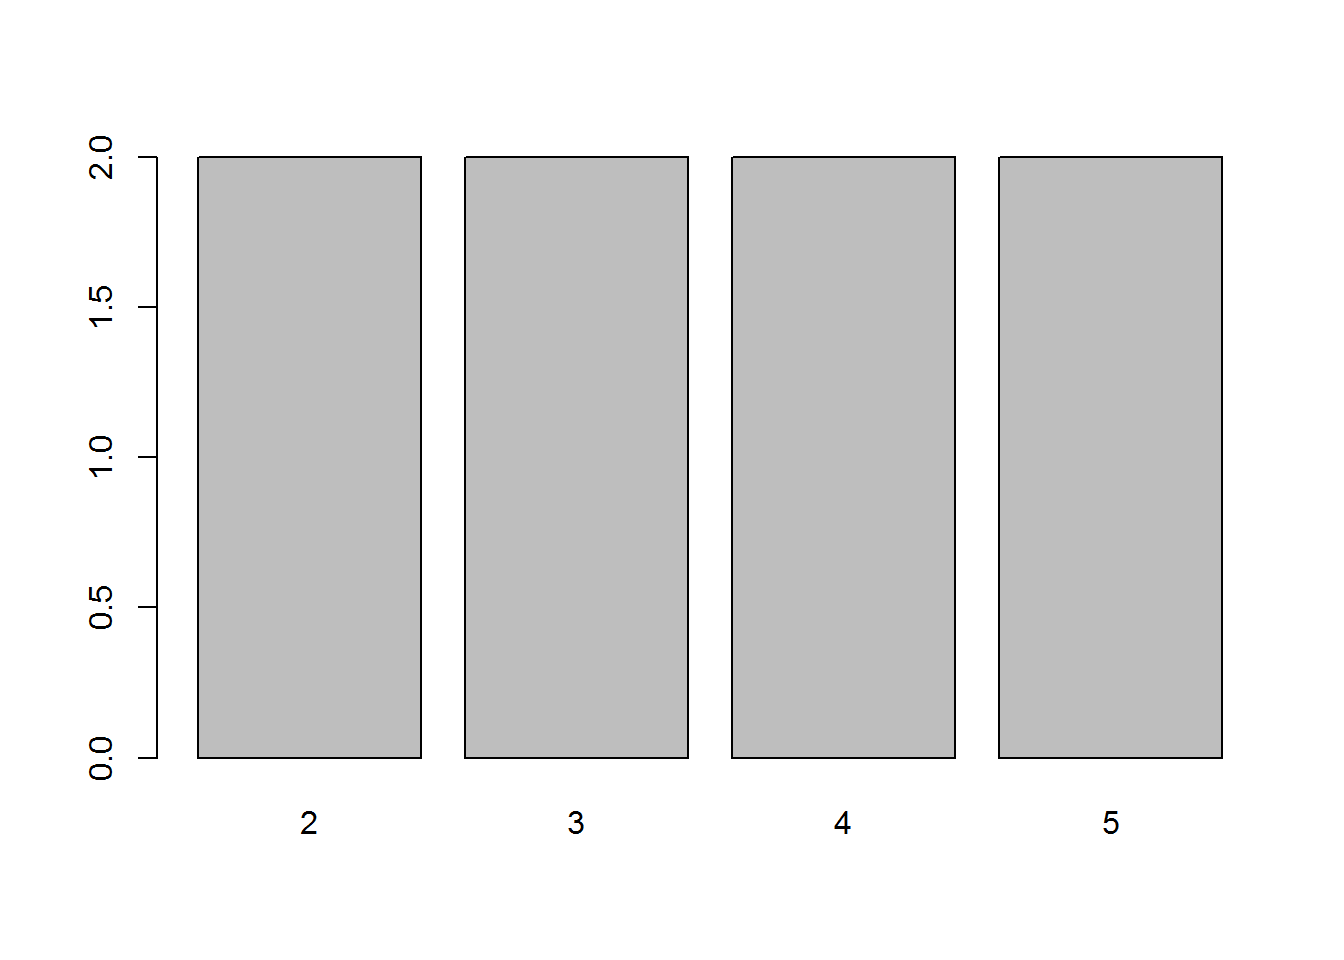
\includegraphics{InferenceStatistique_files/figure-latex/unnamed-chunk-3-1.pdf}
\emph{Tableau 11 : Espace des échantillons}

Bien que la distribution des valeurs dans la population soit plate, la
distribution d'échantillonnage tend vers une distribution normale,
malgré la petite taille de notre population (voir le graphique
ci-dessous).

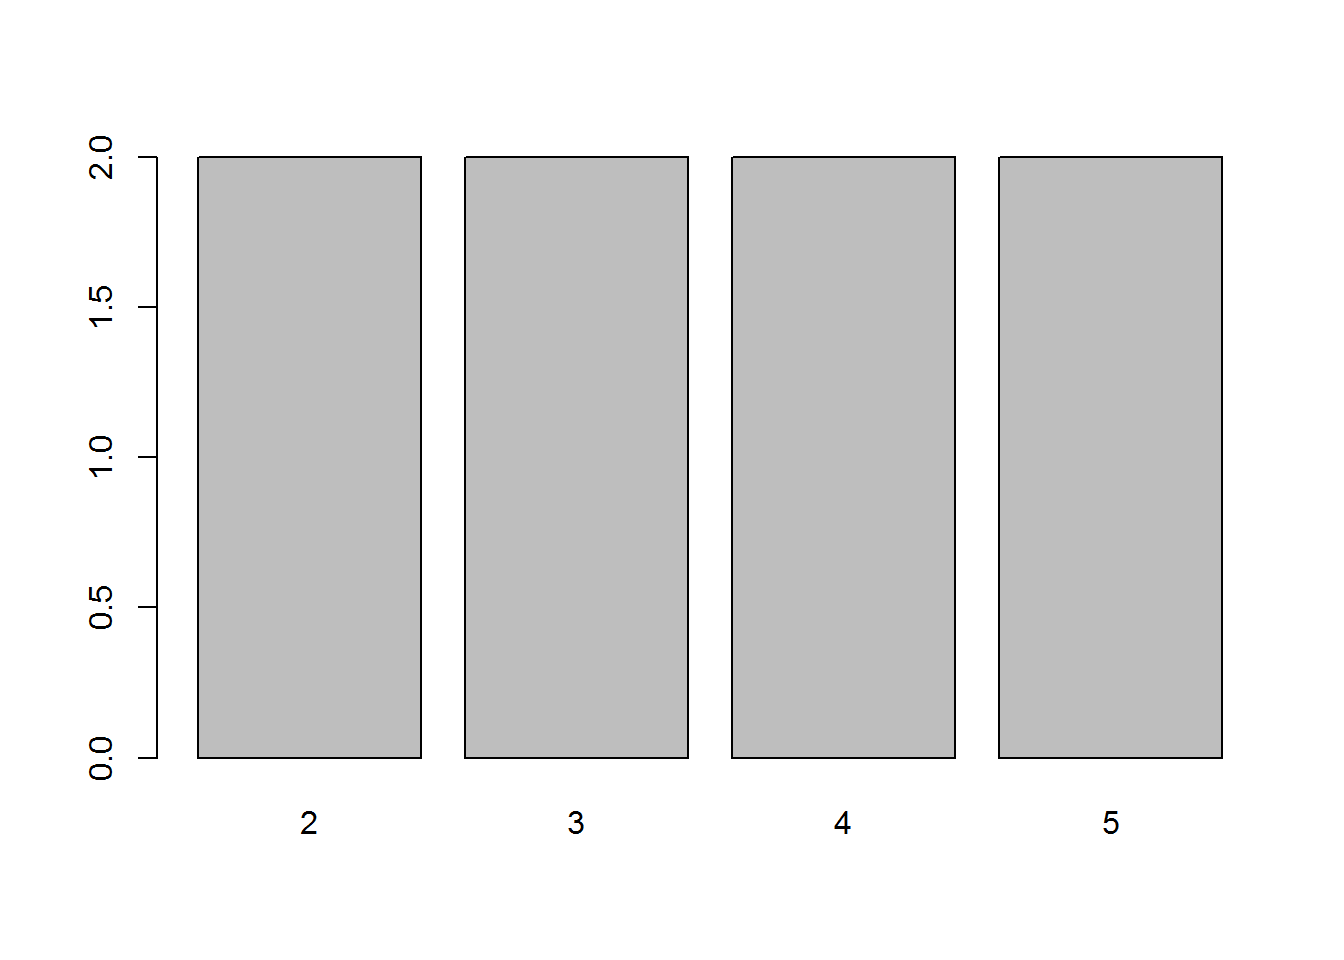
\includegraphics[width=0.5\linewidth]{InferenceStatistique_files/figure-latex/unnamed-chunk-4-1}
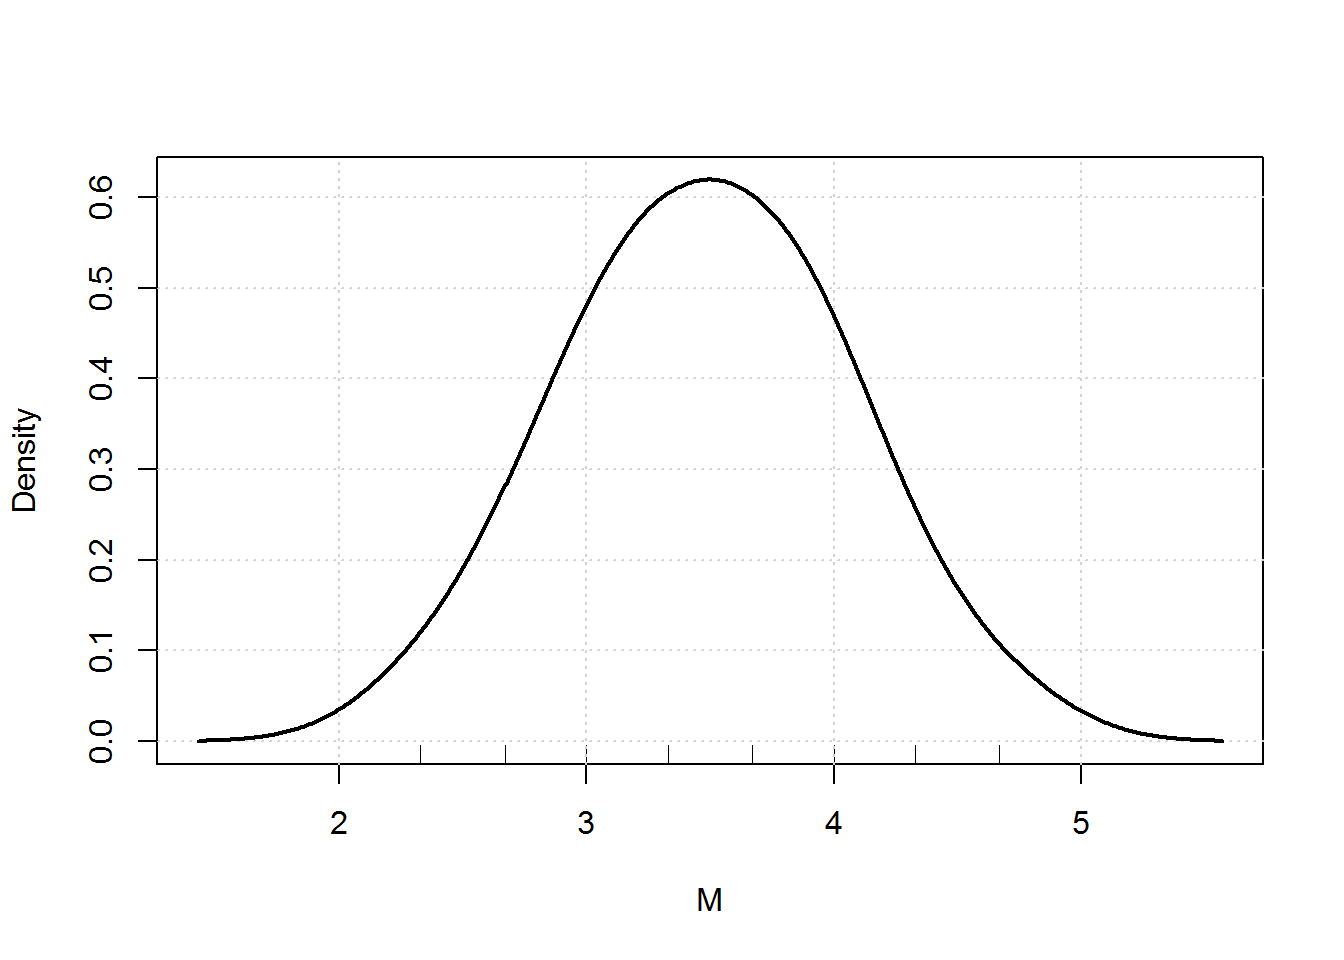
\includegraphics[width=0.5\linewidth]{InferenceStatistique_files/figure-latex/unnamed-chunk-4-2}
\emph{Figure 1 Représentation graphique de la distribution des valeurs
dans la population (graphique de gauche) et de la distribution
d'échantillonnage (graphique de droite)}

Selon le théorème central limite, cette tendance à la normalité de la
distribution d'échantillonnage est d'autant plus marquée que la taille
de la population importante, ce qui va autoriser le recours à des
distributions approchées suivants une loi normale pour l'inférence sur
la moyenne.

\hypertarget{utilisation-dune-distribution-approchee-1}{%
\section{Utilisation d'une distribution
approchée}\label{utilisation-dune-distribution-approchee-1}}

\hypertarget{situer-un-echantillon-dans-une-population-1}{%
\subsection{Situer un échantillon dans une
population}\label{situer-un-echantillon-dans-une-population-1}}

Nous venons de voir que dans le cas de l'échantillonnage dans une
population parente de moyenne \(\mu\) (lire mu) et de variance
\(\sigma ^{2}\) (lire sigma carré), la distribution de la moyenne des
échantillons possibles a également pour moyenne \(\mu\) et pour variance
\(\sigma ^{2}\)/n. Ces propriétés permettent de transformer la
distribution d'échantillonnage en calculant pour chaque valeur de la
moyenne un écart réduit et ainsi d'associer à une distribution des
moyennes, une distribution de Z qui sera également une distribution
normale centrée sur une moyenne 0 et un écart-type de 1. On peut donc,
si on connaît la variance parente, situer notre échantillon dans la
distribution de \(Z\). On peut utiliser cette distribution de \(Z\),
même si la distribution parente n'est pas normale. En effet, on peut
montrer que si le nombre d'observations est assez grand, la distribution
des moyennes des échantillons tend d'autant plus rapidement vers une
distribution normale que n est grand. Concrètement, on peut estimer que
si n est ≥ 20, la distribution \(Z\) est une bonne approximation de la
distribution d`échantillonnage.

Voyons un exemple d'application de ce test. Dans cet exemple de
recherche, on fait passer à l'ensemble des 300 élèves de 3ème d'un
collège, dont 25 étudient le latin, un test de compréhension verbale où
la note représente le nombre de bonnes réponses sur 40 questions. On se
demande si l'étude du latin favorise le développement de ce type de
compétence. Sachant que les latinistes ont obtenu une moyenne de 30 et
l'ensemble des élèves de 3ème, une moyenne de 28 et une variance de 25,
peut-on dire que les latinistes ont une meilleure réussite à ce test ?

Notre population parente est constituée des 300 élèves de 3ème. Notre
échantillon est constitué des élèves latinistes qu'on cherche à situer
dans la population. D'un point de vue psychologique, on se demande si
l'étude du latin favorise le développement des compétences verbales
mesurées par le test. Si tel est le cas, la performance des latinistes à
ce test devrait être supérieure à celles du reste de la population. La
moyenne obtenue par les latinistes est une des moyennes possibles dans
la distribution d'échantillonnage. Mais si le nombre d'échantillons
présentant une moyenne supérieure ou égale à celle de nos latinistes est
suffisamment faible, on pourra considérer que les latinistes font
exception dans la distribution des moyennes au test. Autrement dit, que
les latinistes sont atypiques, du côté des valeurs élevées, de la
population ayant passé le test.

Concrètement, la distribution d'échantillonnage sur les moyennes est
déterminée par la moyenne et l'écart-type. C'est pourquoi on parle
parfois à propos des tests d'inférences sur la moyenne ayant recours à
une distribution approchée normale, de tests paramétriques. Dans cet
exemple, On en connaît la moyenne et la variance qui sont respectivement
de 28 et 25, et on sait que les 25 latinistes ont obtenu une moyenne de
30 au test. La mise en œuvre de ce test commence par le calcul de la
valeur de z correspondant à notre échantillon. Cette valeur est appelée
zobs. La formule est la suivante :

\(z_{obs}=\frac{(m-\mu _{0})}{\sigma _{0}/\sqrt{n}}\)

où m est la moyenne de l'échantillon, \(\mu\) est la moyenne parente et
\(\sigma_{0}\),la variance parente. On peut l'instancier avec les
valeurs de notre exemple ;

\(z_{obs}=\frac{(m-\mu _{0})}{\sigma _{0}/\sqrt{n}}=\frac{30-28}{5/\sqrt{25}} = 2\)

La lecture de la table du \(z\) se fait en recherchant dans la table la
valeur de \(z_{obs}\) et en lisant la proportion associée. De nombreux
manuels présentent trois tables de la loi normale réduite: l'une cumulée
à gauche, une autre cumulée à droite et enfin une table cumulée
bilatérale.

\begin{itemize}
\tightlist
\item
  Si l'hypothèse de recherche à tester situe l'échantillon du côté des
  valeurs basses, il faut utiliser la table cumulée à gauche.
\item
  Si au contraire l'hypothèse situe l'échantillon du coté des valeurs
  hautes, il faut alors utiliser la table cumulée à droite.
\item
  Dans le cas où l'hypothèse est non-orientée, on utilisera la table
  bilatérale.
\end{itemize}

Dans notre exemple, nous faisons l'hypothèse que les latinistes ont une
meilleure performance au test. On cherche donc à savoir s'ils se situent
du coté des valeurs hautes. Il faut donc regarder la distribution
cumulée à droite. La proportion que nous lisons dans la table en regard
de 2 est de .022. Elle représente la proportion des échantillons dans
lesquels la valeur de \(z\) est supérieure à 2. Cette proportion étant
inférieure au seuil repère de .025, le test peut être déclaré
significatif.

L'interprétation du test dépend du modèle d'échantillonnage. Dans
l'approche combinatoire, il s'agit de tester la typicité du groupe
d'observations dans la population. Autrement dit, il s'agit de savoir si
les latinistes sont ou non typiques de la population des élèves de
troisième du point de vue de ce test de compréhension verbale. Le
résultat étant significatif, l'échantillon doit être déclaré atypique de
la population.

On ne peut guère se placer du point de vue fréquentiste dans cette
recherche, dans la mesure où les sujets composant l'échantillon ne
peuvent pas être considérés comme sélectionnés au hasard. On ne peut pas
non plus considérés que toutes choses égales par ailleurs, ces élèves se
différencient des autres uniquement par l'étude du latin. La proportion
ne peut donc pas être interprétée comme une probabilité d'obtenir un tel
échantillon dans la population. D'un point de vue psychologique, la
différence significative nous conduit à affirmer que les compétences
verbales ciblée par le test de compréhension sont plus importantes dans
le cas de l'étude du latin en 3ème.

\hypertarget{situer-un-echantillon-dans-une-distribution}{%
\subsubsection{Situer un échantillon dans une
distribution}\label{situer-un-echantillon-dans-une-distribution}}

Lorsqu'on cherche à situer un échantillon dans une distribution, deux
cas peuvent se présenter :

\begin{itemize}
\tightlist
\item
  soit la variance parente est connue et dans ce cas on est ramené au
  cas précédent dans lequel la distribution approchée à utiliser est
  celle de \(Z\).
\item
  soit la distribution parente n'est pas connue et dans ce cas, la
  distribution approchée à utiliser est la distribution de \(T\) de
  Student.
\end{itemize}

En effet, dans le cas où la variance parente n'est pas connue, le test
du \(Z\) n'est pas utilisable. On peut cependant estimer la variance
parente en calculant la variance corrigée. On peut alors remplacer la
variance parente dans la formule par la variance corrigée. Rappelons que
la variance corrigée est la somme des carrés des écarts à la moyenne
divisée par n-1. On obtient donc la formule suivante :

\(t_{obs}=\frac{()m-\mu _{0})}{s/\sqrt{n}} \textrm { avec } s^{2}=\frac{\sum (x-m)^{2}}{n-1}\)

La démarche est alors la même que dans le cas du \(Z\). La statistique
ainsi calculée est la statistique \(T\). Il s'agit également d'un écart
réduit. La distribution de la statistique \(T\) est un peu différente de
celle du \(Z\). Elle suit une distribution de t de Student à \(\nu\)
(nu) égal n-1 degrés de liberté. Les degrés de liberté correspondent au
nombre de comparaisons binaires qu'on peut faire sur un groupe
d'observations. Dans ce cas,\(\nu\) est égale au nombre d'observations
moins 1. Nous reviendrons sur cette notion dans le cours troisième
année. On estimera la proportion recherchée à l'aide de la table de la
distribution du t de Student.

Pour illustrer l'application du test du t de Student, nous allons
reprendre l'exemple de J-F Richard (1999) sur l'étude de l'illusion de
Muller-Lyer. Cette illusion consiste à percevoir plus grand un segment
encadré par des chevrons intérieurs qu'un segment de même longueur
encadré par des chevrons extérieurs, comme le montre la Figure 2.

\begin{figure}
\centering
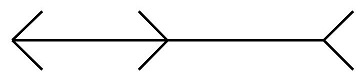
\includegraphics{MullerLyer.jpg}
\caption{Figure 2 L'illusion de Muller-Lyer}
\end{figure}

L'étude de cette illusion se fait en demandant aux sujets d'ajuster la
seconde droite de sorte qu'elle apparaisse de même longueur que la
première. On mesure alors la différence entre la longueur réelle du
second segment et la longueur proposée par le sujet. Sur un groupe de 8
sujets, on a observé que l'estimation était en moyenne supérieure de 2,6
mm par rapport à la longueur réelle, avec un écart-type corrigé de 1,8.
Nous allons dans un premier temps calculer la valeur de tobs sur les
données observées.

\(t_{obs} = \frac{m-\mu _{0}}{s/\sqrt{n}} = \frac{(2,6-0)}{1,8/\sqrt{8}} = 4,09\)

La moyenne observée est de 2,6. La moyenne théorique correspond au cas
où les sujets estimeraient correctement la longueur du second segment,
c'est-à-dire ajusteraient un second segment de même longueur que le
premier. Dans ce cas, l'écart observé serait de 0. L'écart-type corrigé
est de 1,8, et le nombre d'observations est de 8, puisque nous avons 8
sujets et une seule variable. Ce qui nous fait un tobs de 4,09. Il faut
ensuite lire la proportion recherchée dans la table du t de Student. En
tête de colonne de cette table, on trouve les proportions
d'échantillons. La distribution du t de Student étant à peu près
normale, comme celle du Z, la distribution est symétrique. Les
proportions bilatérales sont donc du double des proportions unilatérales
et la table ne signale que les valeurs absolues du t de Student. La
table nous présente, pour un nombre de degrés de liberté donné la valeur
de t qui est dépassée pour chaque proportion.

unilatéral

0,3

0,2

0,1

0,05

0,025

0,01

0,005

0,001

Bilatéral

0,6

0,4

0,2

0,1

0,05

0,02

0,01

0,002

ddl

1

0,73

1,38

3,08

6,31

12,71

31,82

63,66

318,31

2

0,62

1,06

1,89

2,92

4,30

6,96

9,92

22,33

3

0,58

0,98

1,64

2,35

3,18

4,54

5,84

10,21

4

0,57

0,94

1,53

2,13

2,78

3,75

4,60

7,17

5

0,56

0,92

1,48

2,02

2,57

3,36

4,03

5,89

6

0,55

0,91

1,44

1,94

2,45

3,14

3,71

5,21

7

0,55

0,90

1,41

1,89

2,36

3,00

3,50

4,79

8

0,55

0,89

1,40

1,86

2,31

2,90

3,36

4,50

\ldots{}

\ldots{}

\ldots{}

\ldots{}

\ldots{}

\ldots{}

\ldots{}

\ldots{}

\ldots{}

\emph{Tableau 12 : Illustration de la lecture de la table du t de
Student}

Dans notre exemple, \(t_{obs}\) égale 4,09. Nous avons 8 observations
donc 7 degrés de liberté. C'est donc la ligne 7 qu'il nous faut
regarder. Nous cherchons ensuite sur cette ligne la valeur inférieure ou
égale la plus proche à notre tobs. Cette valeur est de 3,50. Nous
testons l'hypothèse que l'estimation des sujets est supérieure à la
longueur réelle du segment 1. Notre hypothèse est donc orientée du côté
des valeurs élevées. En conséquence, nous regarderons le seuil
unilatéral, et lisons en tête de colonne la proportion recherchée. Elle
est de .005. Cette proportion étant inférieure au seuil repère de .025,
le résultat est déclaré significatif au seuil de .005. La valeur pour ce
seuil étant inférieure à la valeur observée, si nous avions une table
plus précise, nous aurions eu une valeur de p inférieure à .005. C'est
la raison pour laquelle, on voit souvent écrit pour rendre compte du
résultat du test que p est inférieur à .005. Cela ne veut pas dire qu'il
est significatif pour toutes les valeurs de p inférieures à .005, On
voit en effet qu'il ne l'est pas pour un seuil de .001. En fait, avec
une table suffisamment précise ou à l'aide de la fonction « t de Student
» d'un tableur, nous aurions trouvé une valeur de p comprise entre .005
et .001. Dans cet exemple, le tableur nous renverrait une valeur de p de
.002.

L'interprétation d'un point de vue statistique dépend, comme toujours,
du modèle d'échantillonnage dans lequel on s'est placé. Dans ce cas de
figure, outre le modèle combinatoire qui est toujours possible, on peut
se placer dans le cadre d'un modèle fréquentiste. Nous cherchons en
effet à tester une hypothèse : dans l'illusion de Muller-Lyer, les
sujets surestiment la longueur du second segment, ce qui les conduit à
ajuster sa longueur par défaut. Par ailleurs, on peut penser que les
sujets sont tirés au hasard dans la population de référence. Dans le
cadre d'un modèle combinatoire, on peut dire que le groupe de sujets
observé est atypique du côté des valeurs élevées à un seuil de .005.
Dans le cadre d'un modèle fréquentiste, on peut dire que la probabilité
d'observer un tel échantillon dans la population est inférieure à .005.
On peut donc rejeter l'hypothèse nulle. Dans les deux cas, on peut
généraliser l'observation que les sujets surestiment la longueur du
segment de gauche.

\hypertarget{inference-sur-un-protocole-univarie-structure-par-un-croisement}{%
\chapter{INFERENCE SUR UN PROTOCOLE UNIVARIE STRUCTURE PAR UN
CROISEMENT}\label{inference-sur-un-protocole-univarie-structure-par-un-croisement}}

Dans ce chapitre, nous allons voir comment faire une inférence sur un
protocole univarié structuré par un croisement. Ce type de structure est
également appelé plan croisé, plan à groupes appariés ou plan à mesures
répétées. Il correspond à une répétition de mesure sur chacune des
modalités du facteur. Dans le cadre de ce cours, nous ne traiterons que
les plans à un facteur. Les plans à plus d'un facteur seront traités en
troisième année.

\hypertarget{les-permutations}{%
\section{Les permutations}\label{les-permutations}}

Dans le cas des structures de croisement, l'espace des échantillons nous
est donné par l'ensemble des permutations possibles. Dans ce type de
protocole, on a pour chacun des sujets un couple d'observations, puisque
la mesure a été répétée dans deux conditions. D'un point de vue
inférentiel, on cherche alors à tester l'homogénéité des groupes
d'observations. On peut considérer que deux groupes d'observations
appariés sont homogènes si on peut permuter les observations d'un ou
plusieurs couples, sans affecter la statistique d'échantillonnage sur
les différences. L'espace des échantillons est alors défini par
l'ensemble des protocoles qu'on peut obtenir en faisant toutes les
permutations possibles entre les observations.

\hypertarget{calcul-de-la-taille-de-lespace-des-echantillons-1}{%
\subsection{Calcul de la taille de l'espace des
échantillons}\label{calcul-de-la-taille-de-lespace-des-echantillons-1}}

Le nombre de permutations possibles est de \(2^{n}\) où n est le nombre
d'individus. Pour illustrer la mise en œuvre du calcul de la
distribution d'échantillonnage par permutation, nous allons, comme
précédemment prendre un exemple simplifié à l'extrême de façon à
faciliter la compréhension du principe général. Nous considérerons donc
un échantillon de 4 individus. Le calcul de la taille de l'espace des
échantillons ne pose pas de difficulté particulière. Si on considère un
échantillon de 4 individus, nous aurons \(2^{4}=16\) échantillons
possibles.

\hypertarget{determination-de-lespace-des-echantillons-1}{%
\subsection{Détermination de l'espace des
échantillons}\label{determination-de-lespace-des-echantillons-1}}

Considérons par exemple un ensemble de 4 individus. Chacun d'eux est
associé à un couple d'observations obtenu dans un ordre particulier, t1
puis t2. Pour chacun des sujets, on peut conserver l'ordre original, que
nous noterons O ou inverser les observations, ce que nous noterons I.
Posons maintenant un tableau contenant autant de lignes que de
protocoles possibles. Un premier protocole possible est l'ordre original
pour tous les sujets. On peut ensuite inverser les observations du
premier sujet, puis celle du second et ainsi de suite. On passera
ensuite aux protocoles comportant deux inversions et en décalant la
seconde d'un cran jusqu'au bout du tableau. On procédera de même pour
les protocoles comportant trois inversions. Le dernier protocole étant
naturellement celui qui comporte quatre inversions. En procédant ainsi,
on est assuré de ne pas en oublier.

S

S1

S2

S3

S4

1

O

O

O

O

2

I

O

O

O

3

O

I

O

O

4

O

O

I

O

5

O

O

O

I

6

I

I

O

O

7

I

O

I

O

8

I

O

O

I

9

O

I

I

O

10

O

I

O

I

11

O

O

I

I

12

I

I

I

O

13

I

I

O

I

14

I

O

I

I

15

O

I

I

I

16

I

I

I

I

\emph{Tableau 1 Détermination des permutations possibles}

Comme précédemment avec les combinaisons, la détermination des
permutations possibles ne dépend pas de l'échelle de mesure, mais va
servir de support au calcul des différences et de la distribution
d'échantillonnage.

\hypertarget{calcul-de-la-distribution-dechantillonnage-1}{%
\subsection{Calcul de la distribution
d'échantillonnage}\label{calcul-de-la-distribution-dechantillonnage-1}}

\hypertarget{cas-dune-variable-nominale}{%
\subsubsection{Cas d'une variable
nominale}\label{cas-dune-variable-nominale}}

Nous allons illustrer l'application du calcul de la distribution
d'échantillonnage en prenant une des tâches les plus utilisée dans
l'étude du raisonnement : la tâche de Wason. Rappelons que dans cette
tâche, l'expérimentateur énonce aux sujets une règle conditionnelle du
type « Si une carte à une voyelle d'un côté, alors elle a un chiffre
pair de l'autre », puis propose aux sujets 4 cartes en lui demandant de
retourner celles qui sont nécessaires et suffisantes pour décider si la
règle est vraie. La bonne réponse consiste à retourner la carte portant
la voyelle et le chiffre impair. Dans une version thématique, ce sont
des enveloppes qui sont présentées aux sujets en leur demandant de
vérifier la règle « si une enveloppe est cachetée alors elle doit être
timbrée à 5 pences ». La bonne réponse consistant à retourner
l'enveloppe à trois pences et l'enveloppe cachetée. Imaginons qu'on ait
fait passer à quatre sujets ces deux tâches, en commençant par la
version formelle suivie de la version thématique. On note pour chacun
des sujets sa réussite ou son échec à la tâche. Nous allons noter 1 les
cas de réussite et 0 les cas d'échec et construire l'espace des
échantillons.

Espace des échantillons

Protocoles des différences

S1

S2

S3

S4

S1

S2

S3

S4

Somme

(0;1)

(1;1)

(0;1)

(0;1)

-1

0

-1

-1

-3

(1;0)

(1;1)

(0;1)

(0;1)

1

0

-1

-1

-1

(0;1)

(1;1)

(0;1)

(0;1)

-1

0

-1

-1

-3

(0;1)

(1;1)

(1;0)

(0;1)

-1

0

1

-1

-1

(0;1)

(1;1)

(0;1)

(1;0)

-1

0

-1

1

-1

(1;0)

(1;1)

(0;1)

(0;1)

1

0

-1

-1

-1

(1;0)

(1;1)

(1;0)

(0;1)

1

0

1

-1

1

(1;0)

(1;1)

(0;1)

(1;0)

1

0

-1

1

1

(0;1)

(1;1)

(1;0)

(0;1)

-1

0

1

-1

-1

(0;1)

(1;1)

(0;1)

(1;0)

-1

0

-1

1

-1

(0;1)

(1;1)

(1;0)

(1;0)

-1

0

1

1

1

(1;0)

(1;1)

(1;0)

(0;1)

1

0

1

-1

1

(1;0)

(1;1)

(0;1)

(1;0)

1

0

-1

1

1

(1;0)

(1;1)

(1;0)

(1;0)

1

0

1

1

3

(0;1)

(1;1)

(1;0)

(1;0)

-1

0

1

1

1

(1;0)

(1;1)

(1;0)

(1;0)

1

0

1

1

3

\emph{Tableau 2 Illustration du calcul de l'espace des échantillons avec
une variable nominale}

Le premier échantillon est l'échantillon observé, puisque les données
sont toutes dans l'ordre original. Le premier sujet a échoué à la tâche
formelle, mais réussi la tâche thématique. Le second a réussi les deux
tâches. Le troisième et le quatrième n'ont réussi que la tâche
thématique. Ensuite, on procède aux permutations indiquées dans le
tableau des permutations. On obtient ainsi les 16 échantillons
possibles. On calculera ensuite, pour chacun des échantillons, le
protocole des différences, en faisant la différence entre la première et
la seconde observation. Dans le premier échantillon, pour le sujet 1,
nous avons 0 pour première observation et 1 pour la seconde. Ce qui nous
donne une différence de -1. Pour le sujet 2, la différence est nulle et
on a -1 pour les sujets 3 et 4. On procède ainsi pour tous les
échantillons possibles. On calcule ensuite pour chacun des échantillons,
la somme des différences. Dans cet exemple, une somme des différences
négative indique une meilleure réussite de la tâche thématique, tandis
qu'une différence positive indique une meilleure réussite de la tâche
formelle. Nous avons ainsi une nouvelle variable dont nous allons faire
la distribution. Pour faire la distribution, il suffit d'ordonner les
sommes des différences et de compter le nombre d'occurrences pour
chacune des modalités de la variable.

Différences

Effectifs

Fréquences

-3

2

0,125

-1

6

0,375

1

6

0,375

3

2

0,125

Total

16

1

\emph{Tableau 3 distribution d'échantillonnage}

Voici la distribution des sommes des différences pour notre exemple.
Nous cherchons à situer le premier protocole. La somme des différences
pour ce protocole est de -3. On peut voir qu'il est présent avec une
fréquence de 0,125 dans l'espace des échantillons. Cette proportion
étant supérieure au seuil repère de .025, le résultat est non
significatif. On peut considérer que l'échantillon observé n'est pas
atypique de la population. Bien sûr, dans cet exemple très artificiel,
et que nous présentons uniquement à des fins d'illustration de la
démarche, aucun échantillon ne peut être déclaré atypique, puisqu'aucune
fréquence n'est inférieure au seuil repère. Il faut rappeler que ces
procédures, comme toutes les procédures statistiques, sont adaptées pour
les grands effectifs que nous n'avons pas pu considérer ici, faute de
place.

\hypertarget{cas-dune-variable-numerique}{%
\subsubsection{Cas d'une variable
numérique}\label{cas-dune-variable-numerique}}

Nous allons voir maintenant une application à une variable numérique.
Dans ce cas, la statistique d'échantillonnage est la moyenne. La
procédure de calcul est analogue à celle que nous avons vu pour les
variables nominales. Posons d'abord un contexte, pour donner du sens à
ce que nous faisons. Pour cela, imaginons que nous avons réalisé une
tâche d'amorçage. On parle d'amorçage lorsque la vitesse
d'identification d'un mot, appelé cible, est influencée par la
présentation préalable d'un autre mot, appelé amorce. Dans ce type
d'expérience, on fait varier la relation sémantique entre l'amorce et la
cible pour mesurer l'effet de cette relation. L'effet d'amorçage dans un
couple amorce-cible est mesuré par différence avec une situation neutre
sans amorce. Nous avons donc deux tâches pour chacun de nos sujets :
identifier la cible avec ou sans amorce. Nous sommes donc bien dans le
cas d'un croisement. Encore une fois, pour des raisons de simplification
et de place, nous nous limiterons à un échantillon de quatre sujets.
Voici l'espace des échantillons.

Espace des échantillons

Protocoles des différences

S1

S2

S3

S4

S1

S2

S3

S4

Somme

(22;17)

(23;11)

(21;10)

(23;12)

5

12

11

11

9,75

(17;22)

(23;11)

(21;10)

(23;12)

-5

12

11

11

7,25

(22;17)

(11;23)

(21;10)

(23;12)

5

-12

11

11

3,75

(22;17)

(23;11)

(10;21)

(23;12)

5

12

-11

11

4,25

(22;17)

(23;11)

(21;10)

(12;23)

5

12

11

-11

4,25

(17;22)

(11;23)

(21;10)

(23;12)

-5

-12

11

11

1,25

(17;22)

(23;11)

(10;21)

(23;12)

-5

12

-11

11

1,75

(17;22)

(23;11)

(21;10)

(12;23)

-5

12

11

-11

1,75

(22;17)

(11;23)

(10;21)

(23;12)

5

-12

-11

11

-1,75

(22;17)

(11;23)

(21;10)

(12;23)

5

-12

11

-11

-1,75

(22;17)

(23;11)

(10;21)

(12;23)

5

12

-11

-11

-1,25

(17;22)

(11;23)

(10;21)

(23;12)

-5

-12

-11

11

-4,25

(17;22)

(11;23)

(21;10)

(12;23)

-5

-12

11

-11

-4,25

(17;22)

(23;11)

(10;21)

(12;23)

-5

12

-11

-11

-3,75

(22;17)

(11;23)

(10;21)

(12;23)

5

-12

-11

-11

-7,25

(17;22)

(11;23)

(10;21)

(12;23)

-5

-12

-11

-11

-9,75

\emph{Tableau 4 Illustration du calcul de l'espace des échantillons avec
une variable numérique}

Comme précédemment, pour la variable nominale, la première ligne
correspond à l'échantillon observé. Les temps de réponses sont donnés en
centièmes de seconde. Le premier chiffre, avant la barre de fraction,
indique le temps de réponse pour les stimuli neutres, c'est-à-dire sans
amorce. Le second chiffre, indique le temps de réponse pour les stimuli
comportant une amorce. Les protocoles des différences sont construits de
la même manière que précédemment, c'est-à-dire en faisant la différence
entre la première et la seconde observation. Dans cet exemple, la
différence représente l'ampleur de l'effet de l'amorce sur la cible. On
calcule ensuite notre statistique d'échantillonnage pour chacun des
protocoles des différences. Dans le cas des variables numériques, cette
statistique est la moyenne, et non la somme qui est utilisée pour les
variables nominales. Le calcul de la distribution d'échantillonnage se
fera de la même façon que précédemment, en ordonnant les moyennes des
différences et en dénombrant les occurrences pour chacune des valeurs.
Voici la distribution d'échantillonnage obtenue sur notre exemple.

Différences

Effectifs

Fréquences

-9,8

1

0,0625

-7,3

1

0,0625

-4,3

2

0,125

-3,8

1

0,0625

-1,8

2

0,125

-1,3

1

0,0625

1,3

1

0,0625

1,8

2

0,125

3,8

1

0,0625

4,3

2

0,125

7,3

1

0,0625

9,8

1

0,0625

Total

16

1

\emph{Tableau 5 Distribution d'échantillonnage}

Dans l'échantillon observé, nous avons une moyenne des différences de
9,8. On peut lire la proportion d'échantillon de même moyenne à la
dernière ligne du tableau de distribution. On voit que cette proportion
est de 0,06, elle est supérieure à notre seuil repère de .025. Le
résultat est donc non significatif. Notre échantillon n'est pas atypique
de la population. Comme dans l'exemple précédent, le nombre de sujets
est trop petit pour qu'un résultat significatif puisse être trouvé et il
s'agit uniquement d'illustrer la démarche.

\hypertarget{interpretation-du-test}{%
\subsubsection{Interprétation du test}\label{interpretation-du-test}}

Quel sens donner au résultat de ce test ? Sans doute ne l'avez-vous pas
remarqué, mais les distributions d'échantillonnage que nous venons de
calculer ont toutes les deux pour moyenne 0. Il en est toujours ainsi.
Les distributions d'échantillonnage de toutes les permutations possibles
sont toujours centrées sur 0. En situant un échantillon dans une telle
distribution, nous nous demandons s'il est atypique d'une distribution
où il n'y a pas de différence entre les deux tâches. L'interprétation du
résultat du test dépend comme toujours du modèle d'échantillonnage
adopté.

Dans le cas d'un modèle combinatoire, dire qu'un échantillon des
différences entre deux tâches est typique d'une distribution des
différences centrée sur 0, c'est dire que les observations dans les deux
tâches sont homogènes, autrement dit qu'on peut mélanger les
observations des deux tâches.

Dans le cadre du modèle fréquentiste, la proportion est interprétée
comme une probabilité d'obtenir l'échantillon observé dans une
distribution de moyenne des différences nulle. On dit qu'on teste
l'hypothèse nulle. Une probabilité supérieure au seuil conduit à ne pas
rejeter l'hypothèse nulle, le risque de se tromper est trop grand. A
l'inverse, une probabilité inférieure au seuil conduit à rejeter
l'hypothèse nulle. Dans ce cas, le risque de se tromper est suffisamment
petit pour qu'on puisse l'accepter.

Comment formulerions-nous la conclusion dans nos deux exemples ? Dans le
cas de la tâche de Wason, une différence négative indique une meilleure
réussite de la tâche thématique. Dans l'échantillon observé, trois
sujets sur quatre échouent à la tâche formelle et réussissent la tâche
thématique. Peut-on dire alors que la tâche thématique est mieux réussie
que la tâche formelle? Si c'est le cas, les observations dans les deux
tâches sont hétérogènes. L'analyse des résultats nous conduit à affirmer
que ce n'est pas le cas.

Dans le second exemple, une différence positive, comme celle de notre
échantillon, reflète l'effet d'amorçage, c'est-à-dire le gain de
rapidité de la réponse dû à la présence de l'amorce avant la cible. Si
l'amorce n'a aucun effet, les observations sur les deux tâches sont
homogènes. Dans cet exemple, on peut effectivement conclure à
l'homogénéité des observations.

\hypertarget{inference-sur-un-protocole-univarie-nominal}{%
\section{Inférence sur un protocole univarié
nominal}\label{inference-sur-un-protocole-univarie-nominal}}

\hypertarget{utilisation-dune-distribution-exacte-2}{%
\subsection{Utilisation d'une distribution
exacte}\label{utilisation-dune-distribution-exacte-2}}

La comparaison de deux groupes d'observations appariés se pose
différemment selon que la variable dépendante à deux ou plus de deux
modalités. Dans le premier cas, le problème revient à se demander si
l'observation est la même dans les deux conditions. Dans le second cas,
cela revient à se demander s'il existe une relation entre les
observations dans la première condition et les observations dans la
seconde, ce qui n'est pas formellement différent de la façon de traiter
un protocole bivarié qui sera abordé au chapitre 5. Nous ne traiterons
donc, dans ce paragraphe, que du cas des variables dépendantes
dichotomiques.

Dans le cas d'un protocole structuré par un croisement avec une variable
nominale dichotomique, la distribution exacte nous est donnée par la
distribution binomiale que nous avons présentée précédemment
(\textbf{voir CHAPITRE 2 - 2.1.2}). Nous avons en effet deux événements
possibles (égalité ou différence des observations dans les deux
conditions) et l'hypothèse d'homogénéité des groupes d'observations (ou
l'hypothèse nulle dans l'approche fréquentiste) revient à postuler une
égalité des fréquences de ces deux événements dans la distribution
d'échantillonnage. Illustrons la démarche d'analyse à l'aide d'une
situation concrète.

Dans une recherche, on souhaite étudier l'effet du nombre de
distracteurs sur la détection de la présence d'un objet cible lors d'une
tâche de détection visuelle. Dans ce type d'expérience, le sujet doit
appuyer sur un bouton à l'apparition d'un objet sur l'écran (cible). Cet
objet est présenté au milieu de plusieurs autres objets (les
distracteurs). On fait l'hypothèse que la cible sera d'autant moins bien
détectée que les distracteurs seront nombreux. Pour cet exemple, nous
allons considérer que 30 sujets doivent détecter la présence d'un objet
cible présenté parmi 20 distracteurs (condition 20) dans une première
condition, et parmi 40 distracteurs dans une seconde condition
(condition 40). La variable dépendante est la détection ou non de la
cible. Le protocole observé est présenté dans le Tableau 6

Pour tester l'hypothèse d'une diminution des détections dans la
condition 40, nous allons considérer la fréquence des individus qui
vérifient l'hypothèse, et la comparer à une fréquence théorique de 50\%
correspondant à une réponse au hasard. Pour cela nous allons recoder les
modalités de la variable en notant 1 les cas de détection et 0 les cas
de non détection. Nous obtenons ainsi une variable pseudonumérique sur
laquelle il est facile de calculer les différences entre la condition 20
et la condition 40. Le protocole recodé et le protocole des différences
est présenté dans le Tableau 6. Dans le protocole des différences, les
différences nulles correspondent aux individus qui ont répondu de la
même façon dans les deux conditions. Du point de vue de notre hypothèse,
ils ne sont pas informatifs. Nous allons donc les ignorer. Les
différences négatives correspondent aux individus dont les réponses
s'opposent à notre hypothèse (non détection en condition 20 et détection
en condition 40). A contrario, les différences positives correspondent
aux individus dont les réponses sont conformes à notre hypothèse
(détection en condition 20 et non détection en condition 40). Ce sont
ces deux derniers que nous allons considérer pour tester notre
hypothèse. C'est ce qu'on appelle le test du signe.

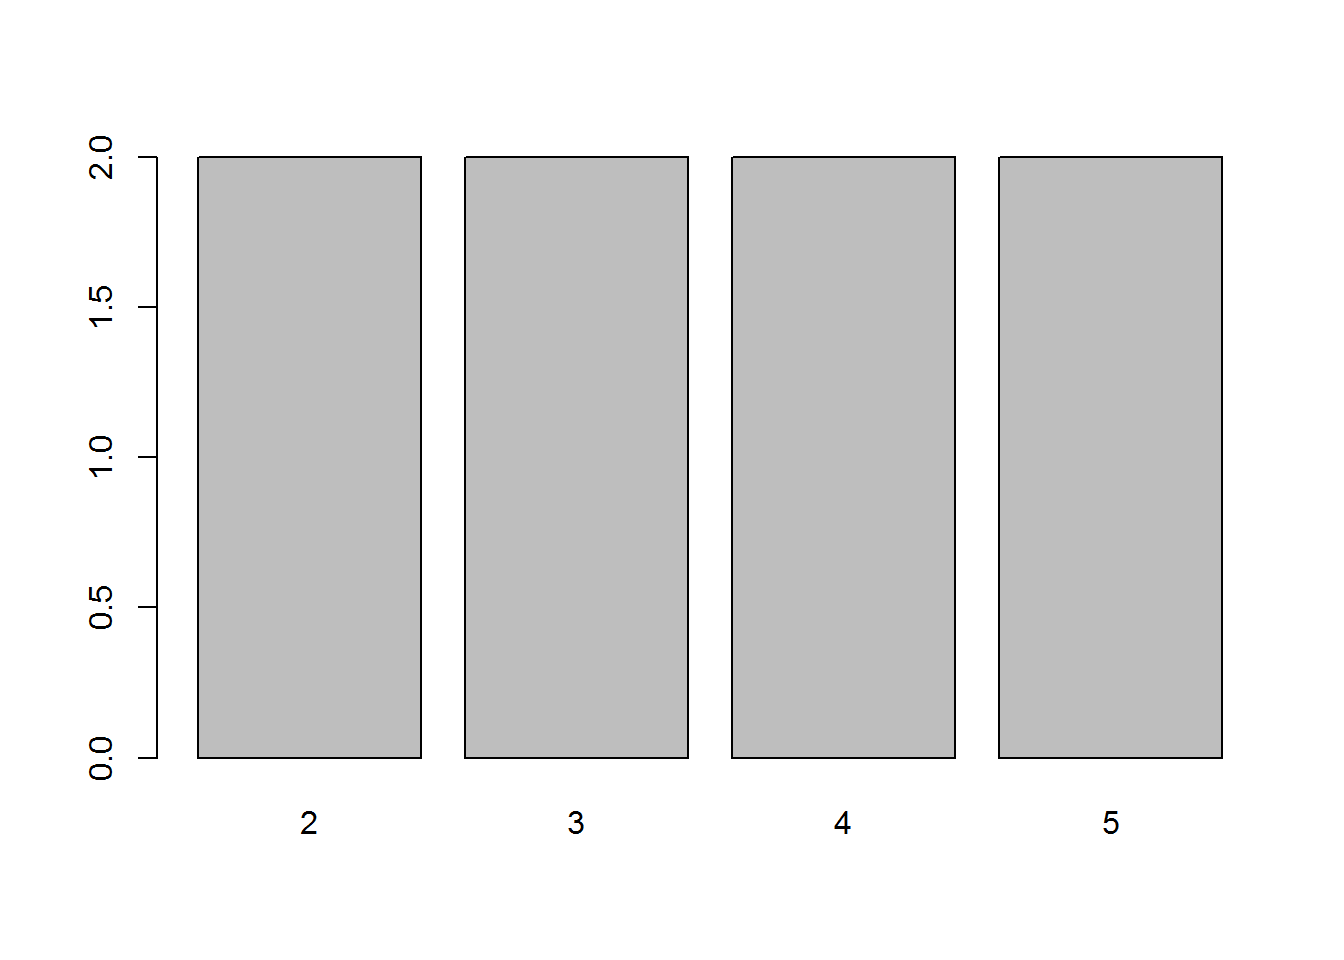
\includegraphics{InferenceStatistique_files/figure-latex/unnamed-chunk-5-1.pdf}

\emph{Tableau 6 Illustration du test du signe}

Si on fait abstraction des cas d'égalité, il nous reste alors 10
individus dont 7 vont dans le sens de l'hypothèse. Nous allons situer
cet échantillon dans une distribution théorique correspondant à des
réponses au hasard, soit une fréquence de détection de 50\%. Il faut
noter qu'en considérant ainsi le protocole des différences, on ramène le
cas de l'inférence sur un protocole structuré par un croisement à celui
de l'inférence sur un protocole univarié non structuré qu'on doit situer
dans une distribution. Ce qui permet de comprendre pourquoi dans ce cas,
la distribution exacte est la distribution binomiale.

Nous avons pour cette distribution les paramètres suivants : \(P=0,5\) ;
\(Q=1-0,5\) et \(n=10\). Il ne nous reste qu'à appliquer la procédure de
calcul présenté précédemment (\textbf{CHAPITRE 2 - 2.1.2}). Les
résultats de ces calculs sont présentés dans le tableau ci-dessous.

\(k\)

\(\binom{n}{k}\)

\(P^{k}\)

\(Q^{n-k}\)

\(p_{k}\)

0

1

1,0000

0,0010

0,001

1

10

0,5000

0,0020

0,010

2

45

0,2500

0,0040

0,044

3

120

0,1250

0,0080

0,117

4

210

0,0625

0,0160

0,205

5

252

0,0313

0,0310

0,246

6

210

0,0156

0,0630

0,205

7

120

0,0078

0,1250

0,117

8

45

0,0039

0,2500

0,044

9

10

0,0020

0,5000

0,010

10

1

0,0010

1,0000

0,001

\emph{Tableau 7 Distribution binomiale}

La première colonne contient les différentes valeurs de k qui vont dans
cet exemple de 0 à 10. On trouve dans la deuxième colonne le nombre de k
éléments dans n éléments (voir le mode de calcul dans le
\textbf{CHAPITRE 2 - 3.2.2)}. Dans la troisième colonne la proportion P
est élevée à la puissance k et dans la troisième colonne Q est élevée à
la puissance n-k. La dernière colonne correspond au produit des trois
précédentes. C'est notre distribution d'échantillonnage. On peut voir
dans cette distribution que la proportion d'échantillons dans lesquels
on a 70\% ou plus d'individus conformes à l'hypothèse est de
0,117+0,044+0,010+0,001=0,172. Cette proportion étant supérieure au
seuil .025, le résultat est donc non significatif. Dans le cadre d'un
modèle d'échantillonnage combinatoire, cela veut dire que le protocole
observé des différences n'est pas atypique d'une distribution où on a
50\% de réponses conformes à l'hypothèse. Autrement dit, les deux séries
d'observations peuvent être considérée comme homogènes. D'un point de
vue fréquentiste, p=0,5 correspond à l'hypothèse nulle, c'est-à-dire
l'absence de différence entre la condition 20 et la condition 40. La
proportion doit alors être interprétée comme la probabilité d'obtenir un
échantillon où il y a 70\% de réponses conformes dans une population où
il y en a 50\%. Cette probabilité étant trop élevée (supérieure au seuil
repère) l'hypothèse nulle n'est pas rejetée. D'un point de vue
psychologique, cela signifie que nos données ne nous permettent pas de
conclure que l'augmentation du nombre de distracteurs diminue la
fréquence de détection de la cible. Cela dépend en fait de la nature des
distracteurs qui, s'ils sont suffisamment différents de la cible,
peuvent même en plus grand nombre favoriser la détection de la cible.
C'est ce qu'on nomme l'effet « pop out ».

\hypertarget{utilisation-dune-distribution-approchee-2}{%
\subsection{Utilisation d'une distribution
approchée}\label{utilisation-dune-distribution-approchee-2}}

La distribution binomiale calculée précédemment peut être approchée à
l'aide d'une distribution de \(\chi ^{2}\) à 1 degré de liberté. Comme
précédemment (voir \textbf{CHAPITRE 2 - 2.2}), cette distribution
approchée peut être utilisée à condition que les effectifs théoriques
soient tous supérieurs à 5 et sous réserve d'appliquer la correction de
continuité. La formule du calcul de \(\chi ^{2}\) est alors la suivante
:

\hypertarget{utilisation-du-test-du-signe}{%
\subsubsection{Utilisation du test du
signe}\label{utilisation-du-test-du-signe}}

Comme précédemment, le test du signe consiste à ne considérer que les
différences non nulles et à situer le protocole des différences dans la
distribution d'échantillonnage. Pour l'utilisation de \(\chi ^{2}\),
cela revient à construire la distribution des effectifs observés en
recodant les données selon trois modalités : les différences conformes à
l'hypothèse, les différences nulles et les différences non conformes à
l'hypothèse. Dans l'exemple précédent, nous avons ainsi la distribution
observée suivante :

Différences

Conformes

Nulles

Non conformes

Total

7

20

3

30

\emph{Tableau 8 Distribution des différences observées}

Les différences nulles n'étant pas informatives du point de vue de
l'hypothèse à tester, on peut en faire abstraction. Nous obtenons ainsi
les effectifs observés suivants où les différences conformes
correspondent au cas de détection dans la condition 20 et de non
détection dans la condition 40. Les différences conformes correspondant
à l'inverse.

Différences obervées

Conformes

Non conformes

Total

7

3

10

\emph{Tableau 9 Illustration du test du signe avec la distribution de}
\(\chi ^2_{[1]}\)

Les effectifs théoriques correspondent à une fréquence des différences
conformes de 0,5 et une fréquence des différences non conformes de
1-0,5=0,5. Nous avons donc comme effectifs théoriques : 10*0,5 soit 5.
Les effectifs théoriques étant supérieurs ou égaux à 5, nous pouvons
calculer \(\chi ^2_{corr}\) :

\(\chi_{corr}^{2} = \frac{(\left | 7-5 \right |-0.5)^{2}}{5}+\frac{(\left | 3-5 \right |-0.5)^{2}}{5}=0.9\)

On consulte ensuite la table de \(\chi ^2_{[1]}\), en cherchant la
valeur la plus proche mais inférieure à la valeur observée. Dans notre
exemple, c'est la valeur .45, ce qui nous permet de lire en tête de
colonne une valeur de p de .05. Le test peut donc être déclaré non
significatif puisque p est supérieur au seuil repère .05 (notre table
est bilatérale). Notre table étant imprécise, l'approximation de p est
grossière. En fait la valeur de p que nous cherchons est comprise entre
.50 et .30 qui correspondent aux valeurs immédiatement inférieures et
supérieures à la valeur observée. Mais un logiciel de statistiques ou
simplement un tableur nous renverrait une valeur de p de 0,34 ce qui
correspond bien au double de ce que nous avons calculer avec la
distribution binomiale.

ddl

0,9

0,8

0,7

0,5

0,3

0,2

0,1

0,05

0,025

0,01

0,001

1

0,02

0,06

0,15

0,45

1,07

1,64

2,71

3,84

5,02

6,63

10,83

2

0,21

0,45

0,71

1,39

2,41

3,22

4,61

5,99

7,38

9,21

13,82

3

0,58

1,01

1,42

2,37

3,66

4,64

6,25

7,81

9,35

11,34

16,27

\ldots{}

\ldots{}

\ldots{}

\ldots{}

\ldots{}

\ldots{}

\ldots{}

\ldots{}

\ldots{}

\ldots{}

\ldots{}

\ldots{}

\emph{Tableau 10 Lecture de la table de \(\chi ^2_{[1]}\)}

\hypertarget{utilisation-du-test-de-mc-nemar}{%
\subsubsection{Utilisation du test de Mc
Némar}\label{utilisation-du-test-de-mc-nemar}}

On peut également utiliser dans le cas d'un protocole structuré par un
croisement avec un facteur à deux modalités, on peut également utiliser
le test de Mc Némar. Ce test est équivalent au test du signe que nous
venons de voir. Il faut pour cela construire un tableau de distribution
croisée à quatre cases. Dans notre exemple, celui-ci se présente ainsi :

Condition 40

Non détection

Détection

Condition 20

Détection

\begin{enumerate}
\def\labelenumi{(\Alph{enumi})}
\tightlist
\item
  7

  B (17)

  Non détection

  (C)~~3

  D (3)

  \emph{Tableau 11 Distribution croisée} Comme précédemment, on ne
  considère que les cas où la différence est non nulle, soit les cases A
  et D. Dans le test du signe, l'effectif théorique est égal à (A+D)/2.
  On peut alors simplifier la formule de X2corr utilisée dans le test du
  signe et obtenir une nouvelle formule de calcul :
\end{enumerate}

\(\chi_{corr}^{2} = \frac{(\left | A-(A+D)/2 \right |-0.5)^{2}}{(A+D)/2}+\frac{(\left | (D-(A+D)/2) \right |-0.5)^{2}}{(A+D)/2}= \frac{(\left | A-D \right |-1)^{2}}{A+D}\)

On peut alors vérifier, en remplaçant les lettres A et D par les valeurs
correspondantes, qu'on obtient bien la même valeur pour
\(\chi ^2_{corr}\) :

\(\chi_{corr}^{2} = \frac{(\left | 7-3 \right |-1)^{2}}{7+3} = 0,9\)

Le test de Mc Némar est donc un cas particulier du test du signe. Il ne
permet de tester que le cas où la fréquence théorique est de 0,5. Pour
les cas où la fréquence théorique est différente de 0,5, il faut
utiliser le test du signe. L'utilisation du test de Mc Némar permet
cependant de simplifier les calculs, mais on doit garder à l'esprit que
ce test s'utilise avec les protocoles univariés structurés par un
croisement (groupes appariés) et ne pas confondre ce test avec le calcul
du \(\chi^{2}\) dans le cas des protocoles structurés par un emboîtement
(groupes indépendants).

\hypertarget{inference-sur-un-protocole-univarie-numerique-1}{%
\section{Inférence sur un protocole univarié
numérique}\label{inference-sur-un-protocole-univarie-numerique-1}}

\hypertarget{utilisation-dune-distribution-exacte-3}{%
\subsection{Utilisation d'une distribution
exacte}\label{utilisation-dune-distribution-exacte-3}}

Dans le cas d'un protocole numérique, la distribution d'échantillonnage
exacte peut être calculée sur l'espace des échantillons déterminé par
combinatoire en cherchant l'ensemble des permutations possibles. Cette
procédure a été développée précédemment (\textbf{CHAPITRE 3 - 1.3.2}).
Nous n'y reviendrons pas.

On peut également utiliser, notamment lorsque la distribution observée
est trop asymétrique, la distribution binomiale en recodant la variable
en ne considérant que le sens des différences. On peut alors mettre en
œuvre le test du signe tel que nous l'avons présenté précédemment. Nous
allons illustrer rapidement cette seconde démarche. Nous allons, pour
cela, reprendre l'exemple de la tâche de détection en imaginant cette
fois que la variable dépendante est le temps de réponse en
millisecondes. L'hypothèse qu'on cherche à tester est que le temps de
détection est plus long avec 40 distracteurs qu'avec 20. Le protocole
observé est donné dans le \textbf{Tableau 12}.

\includegraphics{InferenceStatistique_files/figure-latex/unnamed-chunk-6-1.pdf}
\emph{Tableau 12 Protocole observé et protocole des différences}

A partir du protocole observé, on calcule le protocole des différences.
Ici, nous voulons tester que le temps de réponses est plus long en
condition 40 qu'en condition 20. Nous avons donc fait la soustraction
dans ce sens, de sorte que les différences positives sont celles qui
sont conformes à notre hypothèse et les différences négatives sont
celles qui sont non conformes. Dans la dernière colonne du Tableau 3.12,
nous avons recodé le protocole des différences en ne retenant que le
signe des différences, de sorte que nous obtenons un protocole nominal
qu'il est facile de situer dans une distribution binomiale. Dans cet
exemple n=30 et \(P\) et \(Q\) sont égaux à 0,5.

\(k\)

\(\binom{n}{k}\)

\(P^{k}\)

\(Q^{n-k}\)

p\_\{k\}

25

142506

0,00000030

0,3125

0,000132719

26

27405

0,00000015

0,0625

0,000025523

27

4060

0,00000007

0,125

0,000003781

28

435

0,00000004

0,25

0,000000405

29

30

0,00000002

0,5

0,000000028

30

1

0,00000001

1

0,000000001

\emph{Tableau 3.13 Distribution binomiale}

Nous ne reviendrons pas sur le calcul de la distribution binomiale qui a
déjà été présenté précédemment. Nous présenterons simplement les
résultats. Dans notre exemple, nous cherchons la proportion
d'échantillons pour lesquels on a 25 différences conformes ou plus. Nous
n'avons donc pas besoin de calculer la valeur de pk pour toutes les
valeurs de k. On peut se contenter des valeurs de k≥25. La proportion
que nous cherchons est égale au total de la dernière colonne du
\textbf{Tableau 13}, soit 0,00016. Cette proportion étant inférieure au
seuil repère .025, le résultat peut être déclaré significatif. Les deux
groupes d'observations sont hétérogènes et on peut généraliser le
résultat descriptif d'un temps de réponse dans la condition 40 supérieur
à la condition 20. Dans le cadre d'un modèle d'échantillonnage
fréquentiste, cela signifie que l'hypothèse nulle peut être rejetée.

\hypertarget{utilisation-dune-distribution-approchee-3}{%
\subsection{Utilisation d'une distribution
approchée}\label{utilisation-dune-distribution-approchee-3}}

Comme nous l'avons vu précédemment, avec une variable numérique, deux
distributions approchées peuvent être utilisées : la distribution de
\(Z\) et la distribution de \(T\). Dans le cas où l'échantillon doit
être situé dans une population, la moyenne et la variance parente sont
connues. C'est alors le test du z qui doit être utilisé. Dans le cas où
l'échantillon doit être situé dans une distribution, si la variance
parente est connue c'est également le test du z qui doit être utilisé.
Lorsque la variance parente n'est pas connue, il faut utiliser le test
du t de Student. Dans les deux cas, le principe général de l'inférence
sur un protocole numérique structuré par un croisement consiste à
calculer le protocole des différences et à le situer dans la
distribution d'échantillonnage des différences.

\hypertarget{utilisation-de-la-distribution-du-z}{%
\subsubsection{\texorpdfstring{Utilisation de la distribution du
\(Z\)}{Utilisation de la distribution du Z}}\label{utilisation-de-la-distribution-du-z}}

Pour illustrer la mise en œuvre du test du z, nous allons prendre un
exemple très simplifié. Imaginons que, dans une recherche, on mesure, en
minutes, le temps que les sujets mettent à lire un texte. Puis qu'on
leur donne un second texte traitant du même sujet, présenté
différemment. On fait l'hypothèse que les connaissances acquises au
cours de la lecture du premier texte aideront à la lecture du second. Le
temps de lecture devrait être plus court pour le second texte. On est
dans le cas d'un protocole structuré par un croisement, chaque sujet
ayant vu les deux tâches. Pour comparer le temps moyen de lecture des
deux textes, il faut construire le protocole dérivé des différences
individuelles. Pour cela, on calculera, pour chaque sujet la différence
entre les temps de lecture du premier et du second texte. La dernière
colonne du tableau représente le protocole dérivé des différences
individuelles. En calculant ce protocole, on construit une nouvelle
variable.

Individu

t1

t2

t2-t1

1

8

6

-2

2

6

5

-1

3

4

7

3

4

7

5

-2

5

9

7

-2

6

4

5

1

7

3

4

1

8

6

7

1

9

7

7

0

10

8

6

-2

\emph{Tableau 14 Protocole dérivé des différences} Si on ne considère
que cette dernière variable, on se trouve alors dans le cas d'un
protocole univarié non structuré. Si on connaît la variance parente, on
peut alors utiliser le test du \(z\) tel qu'il a été présenté pour les
protocoles non structurés. Dans cet exemple, la moyenne des différences
de l'échantillon est de -0,3 et l'écart-type des différences est de
1,77.

Imaginons que l'écart-type de la population parente \(\sigma_{0}\) soit
de 1,80. La moyenne parente est de 0. Rappelons que nous testons
l'absence de différences, ce qu'on nomme également l'hypothèse nulle.
Dans notre exemple, l'application de la formule de \(z\) nous donne un
\(z_{obs}\) de :

\(z_{obs} = \frac{m-\mu _{0}}{\sigma _{0}/\sqrt{n}} = \frac{-0,3-0}{1,80/\sqrt{10}} = 0,52\)

La lecture de la table du \(Z\) se fait comme précédemment en
recherchant dans la table la valeur de \(z_{obs}\) et en lisant la
proportion associée. Dans notre exemple, nous faisons l'hypothèse que le
temps de lecture du texte 2 est plus court que le temps de lecture du
texte 1. C'est donc la proportion cumulée à gauche des échantillons que
nous cherchons. La proportion que nous lisons dans la table en regard de
-0,52 est de 0,302. Elle représente la proportion des échantillons dans
lesquels la valeur de Z est inférieure à -0,52. Cette proportion étant
supérieur au seuil repère de .025, le test peut être déclaré non
significatif.

Comme précédemment, l'interprétation du test dépend du modèle
d'échantillonnage dans lequel on se situe. Du point de vue du modèle
combinatoire toujours possible quel que soit le cas de figure, il s'agit
de tester l'homogénéité des deux groupes d'observations. Autrement dit,
si la moyenne des différences est proche de 0, les données des deux
tâches peuvent être mélangées. Le test étant non significatif, les deux
groupes d'observations doivent être considérés comme homogènes.

Dans cet exemple, on peut également se placer dans l'approche
fréquentiste. On teste en effet une hypothèse et on peut considérer, que
toutes choses égale par ailleurs, les deux tâches sont équivalentes. Les
sujets peuvent également être considérés comme tirés au hasard dans la
population. De ce point de vue, la proportion peut alors être
interprétée comme une probabilité d'obtenir une telle moyenne des
différences dans l'espace des échantillons. La probabilité d'obtenir une
moyenne des différences de -0,3 étant trop élevée, on ne peut rejeter
l'hypothèse nulle. Il n'y a donc pas de différence entre les deux
groupes d'observations. On ne peut donc pas dire que la lecture du
second texte soit plus rapide que la lecture du premier. Ce qui d'un
point de vue psychologique pose la question du transfert de connaissance
du premier au second texte.

\hypertarget{utilisation-du-test-du-t-de-student}{%
\subsubsection{Utilisation du test du t de
Student}\label{utilisation-du-test-du-t-de-student}}

Nous allons illustrer l'utilisation du t de Student avec la classique
situation de l'économie au réapprentissage. Dans ce type d'expérience,
l'expérimentateur fait apprendre à deux reprise une liste de mots aux
sujets et mesure le nombre de répétitions nécessaires pour que les
sujets soient capables de restituer parfaitement la liste. La réduction
du nombre de répétition constitue l'économie au réapprentissage.

Imaginons que la liste comporte 20 mots. Dans une première phase, le
sujet doit apprendre la liste par cœur. On mesure le nombre de
répétitions nécessaires à un rappel parfait des 20 mots. Quelques
semaines après, les mêmes sujets sont à nouveau invités à réapprendre la
même liste de mots. On mesure à nouveau le nombre de répétitions
nécessaires pour un rappel parfait de la liste.

Bien qu'avant le deuxième apprentissage, les sujets n'aient pas été
capables de rappeler la liste, on fait l'hypothèse qu'ils n'ont pas
oublié leur premier apprentissage, ce qui devrait se traduire par un
nombre de répétitions nécessaires à un rappel parfait moins important
pour le second apprentissage.

Individu

t1

t2

t2-t1

1

12

10

-2

2

5

7

2

3

11

9

-2

4

11

8

-3

5

11

7

-4

6

6

5

-1

7

14

11

-3

8

14

12

-2

9

9

7

-2

10

11

6

-5

11

9

9

0

12

11

8

-3

\emph{Tableau 15 Dérivation du protocole des différences individuelles}

Nous sommes dans le cas d'un protocole structuré par un croisement,
chaque sujet ayant vu les deux tâches. Pour comparer le nombre de
répétitions dans les deux apprentissages, il faut construire le
protocole dérivé des différences individuelles. Pour cela, on calculera,
pour chaque sujet la différence entre le nombre de répétition au premier
et du second apprentissage. La dernière colonne du tableau représente le
protocole dérivé des différences individuelles. En calculant ce
protocole dérivé, on construit une nouvelle variable. Si on ne considère
que cette dernière variable, on se trouve alors dans le cas d'un
protocole univarié non structuré. Ne connaissant pas la variance
parente, le test du \(Z\) ne peut être employé. Dans ce cas, on
calculera le t de Student. Dans cet exemple, la moyenne des différences
est de 2,08. L'écart-type corrigé des différences est de 1,87. On peut,
à partir de ces paramètres calculer la valeur de \(t_{obs}\).

Rappelons que dans cet exemple, nous testons l'absence de différences,
autrement dit l'hypothèse nulle. La moyenne parente sera donc de 0 et
\(t_{obs}\) est de 3,85.

\(t_{obs} = \frac{m-\mu _{0}}{\sigma/\sqrt{n}} = \frac{2,08-0}{1,87/\sqrt{12}} = 3,85\)

Nous avons 12 observations donc 11 degrés de liberté. C'est donc la
ligne 11 qu'il nous faut regarder. Nous cherchons ensuite sur cette
ligne la valeur inférieur ou égale la plus proche à notre \(t_{obs}\).
Cette valeur est de 3,11. Nous testons l'hypothèse que les sujets font
moins de répétitions lors du second apprentissage pour parvenir à un
rappel parfait.

Notre hypothèse est donc orientée du coté des valeurs basses. En
conséquence, nous regarderons le seuil unilatéral, et lisons en tête de
colonne la proportion recherchée. Elle est de .005. Cette proportion
étant inférieure au seuil repère de .025, le résultat est déclaré
significatif au seuil de .005. La valeur pour ce seuil étant inférieure
à la valeur observée, si nous avions eu une table plus précise, nous
aurions eu une valeur de p inférieure à .005. C'est la raison pour
laquelle, on voit souvent écrit pour rendre compte du résultat du test
que p est inférieur à .005. Cela ne veut pas dire qu'il est significatif
pour toutes les valeurs de p inférieures à .005, On voit en effet qu'il
ne l'est pas pour un seuil de .001. En fait, avec une table suffisamment
précise ou à l'aide de la fonction t de Student d'un tableur, nous
aurions trouvé une valeur de p comprise entre .005 et .001. Dans cet
exemple, le tableur nous renverrait une valeur de p de .0013.

Comme précédemment, l'interprétation d'un point de vue statistique
dépend du modèle d'échantillonnage dans lequel on se place. Du point de
vue du modèle combinatoire, toujours possible quel que soit le cas de
figure, il s'agit de tester l'homogénéité des deux groupes
d'observations. Autrement dit, si la moyenne des différences est proche
de 0, les données des deux tâches peuvent être mélangées. Le test étant
significatif, les deux groupes d'observations doivent être considérés
comme hétérogènes. La valeur de t étant positive, on a
t1\textgreater{}t2. On peut donc dire que les sujets ont besoin de moins
de répétitions, dans le second apprentissage, pour réapprendre
parfaitement la liste de mots.

Dans cet exemple, on peut également se placer dans l'approche
fréquentiste. On peut, en effet, considérer que les sujets sont tirés au
sort dans la population et que toutes choses égales par ailleurs, les
deux tâches sont comparables. De ce point de vue, la proportion p peut
être interprétée comme étant la probabilité d'obtenir une différence de
2,08. Autrement dit, on a 5 chances sur mille d'obtenir un échantillon
présentant une moyenne supérieure ou égale à celle observée dans notre
échantillon. Ce qui permet dans trop de risque de rejeter l'hypothèse
nulle d'absence de différences.

D'un point de vue psychologique, on peut donc généraliser l'idée que les
sujets réapprennent plus vite une liste de mots, même si à première vue
ils ne s'en souviennent pas. Ce qui montre que le premier apprentissage
n'est pas perdu, mais seulement inaccessible en mémoire.

\hypertarget{inference-sur-un-protocole-univarie-structure-par-un-emboitement}{%
\chapter{INFERENCE SUR UN PROTOCOLE UNIVARIE STRUCTURE PAR UN
EMBOITEMENT}\label{inference-sur-un-protocole-univarie-structure-par-un-emboitement}}

\hypertarget{les-partitions}{%
\section{Les partitions}\label{les-partitions}}

Dans le cas des groupes indépendants, c'est-à-dire des protocoles
structurés par un emboîtement, la distribution d'échantillonnage exacte
peut être obtenue par combinatoire en calculant l'ensemble des
partitions possibles. Nous allons comment se fait ce calcul dans le cas
des variables nominales et dans le cas des variables numériques.

\hypertarget{calcul-de-la-taille-de-lespace-des-echantillons-2}{%
\subsection{Calcul de la taille de l'espace des
échantillons}\label{calcul-de-la-taille-de-lespace-des-echantillons-2}}

Dans un protocole structuré par un emboîtement, on teste l'idée que les
groupes sont homogènes, autrement dit que les individus dans chacun des
groupes sont interchangeables. Une autre façon de l'exprimer est de
considérer que les deux groupes sont issus d'une seule et même
population parente. L'échantillon observé constitue donc une des
partitions possibles de la population. L'ensemble des partitions
correspond aux différentes façons de répartir les individus dans les
deux groupes. Le nombre de partitions possibles est donné par la formule
suivante :

\(A_{k}^{n} =\frac{N!}{n!(N-n)!}\)

Le symbole à gauche de l'égalité se lit « nombre de combinaisons de n
éléments dans N éléments ». La formule de droite nous permet de le
calculer. Par exemple, si on cherche à savoir combien de groupes de
trois éléments sont possibles dans une population de 5 éléments, Nous
aurons 10 partitions possibles :

\(\binom{5}{3} = \frac{5!}{3!(5-3)!} = \frac{5*4*3*2*1}{3*2*1*2*1} = 10\)

Conservons pour l'exemple notre population de 5 individus et déterminons
l'ensemble des partitions possibles. Encore une fois, cette procédure
est présentée à titre d'illustration. L'exemple, bien que peu réaliste,
vise plus à vous faire comprendre de quoi il retourne qu'à vous faire
acquérir une procédure qu'en pratique, on utilise rarement. Ce qui
importe donc ici, c'est la démarche d'analyse.

Groupe 1

Groupe 2

Partitions

S1

S2

S3

S4

S5

1

1

2

3

4

5

2

4

2

3

1

5

3

5

2

3

4

1

4

1

4

3

2

5

5

1

5

3

4

2

6

1

2

4

3

5

7

1

2

5

4

3

8

4

5

3

1

2

9

1

4

5

2

3

10

4

2

5

1

3

\emph{Tableau 1 Espace des échantillons possibles}

Nous avons donc 10 échantillons possibles. Posons alors un tableau
comportant 11 lignes, la première indiquant l'identifiant de nos
individus. La première partition est constituée du protocole observé.
Pour constituer une nouvelle partition, on peut échanger le premier
élément du premier groupe avec l'un des éléments de l'autre groupe.
L'élément 1 contre l'élément 4 ou l'élément 1 contre l'élément 5. On
aurait pu également échanger l'élément 2 contre le 4 ou le 5. On peut
faire de même avec l'élément 3. Au lieu d'échanger un seul élément, on
peut également en échanger 2. On peut alors échanger les deux premiers,
les deux derniers ou le premier et le dernier. On ne peut pas, dans cet
exemple, échanger plus de deux éléments puisque le complément n'en
comporte que deux. Nous avons donc l'ensemble des partitions pour nos
deux groupes.

\hypertarget{calcul-de-la-distribution-dechantillonnage-2}{%
\subsection{Calcul de la distribution
d'échantillonnage}\label{calcul-de-la-distribution-dechantillonnage-2}}

\hypertarget{cas-dune-variable-nominale-1}{%
\subsubsection{Cas d'une variable
nominale}\label{cas-dune-variable-nominale-1}}

Comme précédemment, la statistique d'échantillonnage pour une variable
nominale est la fréquence. Celle-ci sera calculée pour l'une des deux
modalités de la variable dans chacun des groupes. Imaginons, pour
l'exemple, que nous ayons deux groupes de sujets, l'un composé de trois
garçons, l'autre de deux filles, et qu'on leur donne une tâche de calcul
mental à réaliser. La réussite sera codée 1, l'échec sera codé 0. Voici
l'espace des échantillons.

Groupe 1

Groupe 2

Fréquences de réussite

Partitions

S1

S2

S3

S4

S5

G1

G2

D

1

1

0

1

0

1

0,67

0,50

0,17

2

0

0

1

1

1

0,33

1,00

-0,67

3

1

0

1

0

1

0,67

0,50

0,17

4

1

0

1

0

1

0,67

0,50

0,17

5

1

1

1

0

0

1,00

0,00

1,00

6

1

0

0

1

1

0,33

1,00

-0,67

7

1

0

1

0

1

0,67

0,50

0,17

8

0

1

1

1

0

0,67

0,50

0,17

9

1

0

1

0

1

0,67

0,50

0,17

10

0

0

1

1

1

0,33

1,00

-0,67

\emph{Tableau 2 Espace des échantillons}

La partition 1 correspond à l'échantillon observé. Nous allons
maintenant calculer pour chaque groupe la fréquence des réussites,
c'est-à-dire le nombre de réussites rapporté au nombre de sujets dans le
groupe. Pour le groupe 1, dans la première partition, nous avons 2
réussites pour trois sujets, soit donc une fréquence de 2/3. Dans le
groupe 2 de la partition 1, nous avons 1 réussite pour 2 sujets, soit
donc une fréquence de 1/2. On calcule ensuite la différence entre ces
deux fréquences. Une différence de fréquences positive nous indique de
G1 \textgreater{} G2, autrement dit que la fréquence de réussite est
plus importante dans le groupe des garçons. Une fréquence négative
indique bien sûr une meilleure performance des filles. Dans
l'échantillon observé, la différence de fréquence est de 0,17. Nous
allons la situer dans la distribution d'échantillonnage.

Comme toujours, la distribution des différences de fréquences se fait en
ordonnant ces différences et en comptant les occurrences pour chaque
valeur. Voici la distribution d'échantillonnage correspondant à notre
exemple.

Différences

Effectifs

Fréquences

-0,67

3

0,3

0,17

6

0,6

1,00

1

0,1

\emph{Tableau 3 Distribution d'échantillonnage des différences de
fréquences}

On peut voir que la proportion des échantillons présentant une
différence de fréquences de 0,17 est de 0,6, proportion bien sûr très
supérieure au seuil repère .025, ce qui est normal, puisque notre
exemple est extrêmement simplifié. On voit en effet que quel que soit
l'échantillon, il n'a, dans cette distribution, aucune chance d'être
atypique. Il faut rappeler que les méthodes statistiques sont adaptées
aux grands groupes de sujets et que sur un exemple comme celui-ci, qui
peut servir à expliquer la démarche, ces méthodes ne sont pas très
pertinentes.

\hypertarget{cas-dune-variable-numerique-1}{%
\subsubsection{Cas d'une variable
numérique}\label{cas-dune-variable-numerique-1}}

Dans le cas des variables numériques, la statistique d'échantillonnage
pertinente est la moyenne. Pour le reste, la démarche est en tous points
analogue à celle employée sur les variables nominales. Prenons un
exemple simple pour illustrer cette démarche en imaginant qu'on est
relevé l'âge de nos sujets. A partir de l'ensemble des partitions
possibles, on déterminera l'espace des échantillons.

Groupe 1

Groupe 2

Fréquences de réussite

Partitions

S1

S2

S3

S4

S5

G1

G2

D

1

8

7

8

7

9

7,67

8,00

-0,33

2

7

7

8

8

9

7,33

8,50

-1,17

3

9

7

8

7

8

8,00

7,50

0,50

4

8

7

8

7

9

7,67

8,00

-0,33

5

8

9

8

7

7

8,33

7,00

1,33

6

8

7

7

8

9

7,33

8,50

-1,17

7

8

7

9

7

8

8,00

7,50

0,50

8

7

9

8

8

7

8,00

7,50

0,50

9

8

7

9

7

8

8,00

7,50

0,50

10

7

7

9

8

8

7,67

8,00

-0,33

\emph{Tableau 4 Espace des échantillons}

Comme précédemment la première partition est le protocole observé. On
calculera ensuite pour chaque groupe la moyenne des âges, puis la
différence entre les moyennes d'âge du groupe 1 et du groupe 2. Une
différence positive signifie que G1\textgreater{}G2, c'est-à-dire dans
ce cas que l'âge moyen des garçons est plus important que celui de
filles. Une différence négative signifie bien sûr le contraire. Il ne
reste plus qu'à situer l'échantillon dans la distribution
d'échantillonnage.

Différences

Effectifs

Fréquences

-0,33

1

0,1

-1,17

2

0,2

-0,33

2

0,2

0,5

4

0,4

1,33

1

0,1

\emph{Tableau 5 Distribution d'échantillonnage des différences}

Cette distribution se fait simplement en ordonnant les différences de
moyennes et en comptant les occurrences pour chaque valeur de la
moyenne. Dans notre exemple, la différence de moyennes est de -0,33, ce
qui signifie que les filles sont plus âgées que les garçons. Cette
différence est observée dans une proportion de 0,1 dans l'espace des
échantillons. Notre échantillon n'est donc pas atypique.

\hypertarget{interpretation-du-test-1}{%
\subsection{Interprétation du test}\label{interpretation-du-test-1}}

Sous réserve que le nombre d'observations soit suffisamment grand, la
distribution des différences de moyennes se centre sur 0. Autrement dit,
ce qu'on cherche à tester en situant un échantillon dans l'ensemble des
partitions possibles, c'est sa typicité dans une population où la
différence entre les deux groupes est nulle. L'interprétation du
résultat dépend du modèle d'échantillonnage dans lequel on se situe.

Dans le cadre de l'inférence combinatoire, cela revient à tester
l'homogénéité entre les deux groupes. Dans nos deux exemples, nous avons
vu que l'échantillon n'est pas atypique de la distribution des
différences entre les deux groupes. Cela revient à dire que les deux
groupes constituant la partition sont homogènes. En effet, comme l'a
montré Rouanet (1990) le test d'homogénéité est formellement équivalent
à un test de typicité si on prend pour population la réunion des deux
groupes.

Dans le cadre de l'inférence fréquentiste, la proportion est interprétée
comme une probabilité d'obtenir la différence des moyennes observée dans
un espace des échantillons centré sur 0, On dit qu'on teste l'hypothèse
nulle. Dans ce cas, une proportion inférieure au seuil repère conduit à
rejeter l'hypothèse nulle et donc à admettre l'existence d'une
différence.

\hypertarget{inference-sur-un-protocole-univarie-nominal-1}{%
\section{Inférence sur un protocole univarié
nominal}\label{inference-sur-un-protocole-univarie-nominal-1}}

\hypertarget{utilisation-dune-distribution-exacte-4}{%
\subsection{Utilisation d'une distribution
exacte}\label{utilisation-dune-distribution-exacte-4}}

Dans le cas d'un plan structuré par un emboîtement sur une variable
nominale, la distribution exacte dépend du nombre de modalités du
facteur. Dans le cas d'un facteur à deux modalités, la distribution
exacte est la distribution hypergéométrique. Dans le cas d'un facteur à
plus de deux modalités, la distribution exacte est une distribution
multinomiale. Seul le premier cas, sera abordé dans le cadre de ce cours
Nous verrons plus loin comment faire une inférence pour les facteurs à
plus de deux modalités en utilisant une distribution d'échantillonnage
approchée.

Catégorie visée

Catégorie complémentaire

Total

Groupe = Echantillon

k

n-k

n

Groupe 2 = Complément

A-k

N-A-(n-k)

N-n

Population

A

N-A

N

\emph{Tableau 4.6 Tableau des paramètres de la distribution
hypergéométrique (à gauche, dans le cas de la comparaison d'un groupe
d'observations à une population ; à droite, dans le cas d'une
comparaison de deux groupes d'observation).}

Dans le cas des groupes indépendants, l'utilisation de la distribution
hypergémoétrique revient en fait à considérer comme population la
réunion des deux groupes pour y situer un des deux groupes. Si le groupe
d'observations considéré est atypique de la la distribution
d'échantillonnage faite sur la réunion des deux groupes, cela revient à
dire que les deux groupes ne sont pas homogènes. Illustrons la démarche
d'un petit exemple.

Dans une recherche sur l'acquisition de l'addition, on fait résoudre un
problème à 40 enfants de CE2. Dans un premier groupe, le problème est
une situation de recherche de l'état final : « Pierre à 3 bonbons, sa
maman lui en donne 5. Combien en a-t-il maintenant ? ». Dans le second
groupe, le problème est une situation de recherche de l'état initial: La
maman de Paul lui donne 5 bonbons, il en a maintenant 8. Combien en
avait-il avant? On fait l'hypothèse que le problème de recherche de
l'état final est plus facile que le problème de recherche de l'état
initial. Pour analyser les données, il faut d'abord construire un
tableau à double entrée en réalisant un tri croisé (voir vos cours de
première année). Voici les données observées dans cet exemple.

Performance

Réussite

Echec

Total

Type de problème

Etat final

16

4

20

Etat initial

7

13

20

Total

23

17

40

\emph{Tableau 7 Effectifs observés pour chaque type de problème} Si nous
prenons comme catégorie visée les réussites en cherchant à situer le
premier groupe dans la réunion des deux groupes, nous allons devoir
calculer la distribution hypergéométrique pour les valeurs de k allant
de 16 à 20. La variable observée ayant deux modalités, la fréquence des
échecs est le complément de la fréquence des réussites. Ainsi, dans la
distribution d'échantillonnage, la proportion d'échantillons présentant
une fréquence des réussites supérieure ou égale à 16/20 est la même que
la proportion d'échantillons présentant une fréquence des échecs
inférieure ou égale à 4/20. Il est donc équivalent de tester
l'homogénéité des groupes d'observations sur les réussites et les
échecs. C'est la raison pour laquelle, en pratique, l'inférence est
faite sur la catégorie présentant l'effectif le plus faible. Dans notre
cas, il vaut mieux faire l'inférence sur les échecs dans le groupe ayant
eu le problème sur l'état final. Le tableau doit alors être posé de la
façon suivante :

Il nous faut alors calculer \(p_{k}\) pour une valeur de k variant de 0
à 4. La procédure de calcul ayant été présenté précédemment
(\textbf{CHAPITRE 2 - 2.1}) nous ne le reprendrons pas ici. Nous nous
contenterons de présenter les résultats des calculs. Rappelons que ce
que nous cherchons ici, c'est la proportion d'échantillons présentant
une fréquence d'échecs inférieures ou égales à 4/20. C'est donc la
proportion cumulé pour les valeurs de k allant de 0 à 4 qu'il nous faut
regarder. Dans notre exemple, cette proportion est de .004, ce qui est
inférieur au seuil repère de .025. Le résultat est donc significatif. Le
groupe ayant eu le problème sur l'état final est atypique de la réunion
des deux groupes du côté des valeurs basses. Cela revient à dire que les
deux groupes sont hétérogènes, le groupe considéré présentant une
fréquence d'échecs plus faible.

\(k\)

\(n-k\)

\(A-k\)

\(N-A-(n-k)\)

\(p_{k}\)

\(p_{k}\) cumulé

0

20

17

3

0,00000001

0,00000001

1

19

16

4

0,00000109

0,00000110

2

18

15

5

0,00003320

0,00003430

3

17

14

6

0,00049797

0,00053228

4

16

13

7

0,00423278

0,00476505

\emph{Tableau 8 Distribution hypergéométrique sur l'exemple de la
résolution de problèmes arithmétiques}

\hypertarget{utilisation-dune-distribution-approchee-4}{%
\subsection{Utilisation d'une distribution
approchée}\label{utilisation-dune-distribution-approchee-4}}

Comme toujours, la distribution approchée dans le cas des variables
nominales est la distribution de \(\chi ^{2}\). Nous devons ici
considérer deux cas de figures : (i) la comparaison de deux groupes
d'observations et (ii) la comparaison de plus de deux groupes
d'observations. Dans le premier cas, l'inférence se fera à l'aide de la
distribution de \(\chi ^{2}\) à 1 degré de liberté. Dans le second,
l'inférence se fera à l'aide de la distribution de \(\chi ^{2}\) à
(k-1)(l-1) degrés de liberté en prenant pour k le nombre de catégorie et
pour l le nombre de groupes.

\hypertarget{comparaison-de-deux-groupes-dobservations}{%
\subsubsection{Comparaison de deux groupes
d'observations}\label{comparaison-de-deux-groupes-dobservations}}

Pour illustrer la comparaison de deux groupes d'observations, nous
allons reprendre l'exemple de la résolution de problèmes arithmétiques.
Rappelons que dans le cas de l'inférence à l'aide de la distribution de
\(\chi ^{2}\) à 1 ddl, deux conditions doivent être respectées : (i)
Tous les effectifs théoriques doivent être supérieures à 5 et (ii) il
faut appliquer une correction de continuité.

Effectifs observés

Performance

Réussite

Echec

Total

Type de problème

Etat final

16

4

20

Etat initial

7

13

20

Total

23

17

40

Effectifs théoriques

Performance

Réussite

Echec

Total

Type de problème

Etat final

11,5

8,5

20

Etat initial

11,5

8,5

20

Total

23

17

40

\emph{Tableau 9 Effectifs observés et théoriques dans l'exemple de la
résolution de problèmes arithmétiques}

Dans un premier temps, nous devons calculer les effectifs théoriques
avant d'appliquer la formule du \(\chi ^{2}\). Dans le cas des groupes
indépendants, nous cherchons à tester l'hypothèse que les fréquences de
chacune des modalités de la variable dépendante sont les mêmes dans les
deux groupes. La fréquence des réussites sur les deux groupes est de
23/40. La fréquence des sujets ayant passé le problème 1 est de 20/40.
L'effectif théorique des réussites dans le groupe 1 est donc de 23*20/40
soit 11,5, autrement dit la moitié de 23, puisque la moitié des sujets
sont dans le groupe 1. Selon le même raisonnement, l'effectif théorique
des échecs dans le même groupe est de 17*20/40=8,5. On devine aisément
que les effectifs théoriques du groupe 2 sont les mêmes. Aucun effectif
théorique n'étant inférieure à 5, on peut maintenant appliquer la
formule du \(\chi ^2_{corr}\).

\(\chi _{corr} ^{2}=\frac{(\left | 16-11,5 \right |-0,5)^{2}}{11,5}+\frac{(\left | 4-8,5 \right |-0,5)^{2}}{8,5}+\frac{(\left | 7-11,5 \right |-0,5)^{2}}{11,5}+\frac{(\left | 13-8,5 \right |-0,5)^{2}}{8,5}=6,55\)

Nous allons situer cette valeur dans la distribution approchée. Dans le
cas de la comparaison de deux groupes d'observations, seule la
distribution de \(\chi ^2\) à 1 ddl nous intéresse. Cette distribution
nous indique, pour chaque valeur de Khi-deux, la proportion
d'échantillons qui dépassent cette valeur.

ddl

.90

.80

.70

.50

.30

.20

.10

.05

.025

.01

.001

1

0,02

0,06

0,15

0,46

1,07

1,64

2,71

3,84

5,02

6,64

10,83

2

0,21

0,45

0,71

1,39

2,41

3,22

4,60

5,99

7,38

9,21

13,83

3

0,58

1,00

1,42

2,37

3,66

4,64

6,25

7,82

9,35

11,34

16,27

\ldots{}

\ldots{}

\ldots{}

\ldots{}

\ldots{}

\ldots{}

\ldots{}

\ldots{}

\ldots{}

\ldots{}

\ldots{}

\ldots{}

\emph{Tableau 10 lecture de la table de \(\chi ^{2}\)}

On peut lire cette proportion dans la première ligne du tableau. La
proportion signalée dans ce tableau est une proportion bilatérale. Le
khi-deux observé est de 6,55. Nous allons chercher dans la table la
valeur inférieure ou égale la plus proche de notre valeur observée.
C'est la valeur 5,02. Elle correspond à une valeur de p de .025. Cette
dernière valeur étant inférieure au seuil repère de .05, le test est
significatif. Comme à chaque fois, l'interprétation du test dépend du
modèle d'échantillonnage dans lequel on se place.

Dans le modèle combinatoire, il s'agit de tester l'idée que les
fréquences de chacune des modalités de la variable dépendante sont les
mêmes dans les deux groupes et donc que les observations des deux
groupes peuvent être mélangées. Autrement dit, on teste l'homogénéité
des groupes. Dans notre exemple, on voit que le résultat est
significatif. Les groupes sont donc hétérogènes.

Dans le cadre de l'inférence fréquentiste, on teste l'hypothèse nulle
d'absence de différences entre les groupes. La proportion est alors
interprétée comme une probabilité d'observer un tel échantillon dans une
population où il n'y aurait pas de différence entre les groupes. La
probabilité est suffisamment faible pour qu'on puisse rejeter
l'hypothèse nulle sans prendre un trop grand risque de se tromper.

D'un point de vue psychologique, la différence significative est à
rapporter aux résultats de l'analyse descriptive qui montrent que la
réussite est plus importante dans le problème portant sur l'état final
que dans le problème sur l'état initial. Ce second problème est donc
beaucoup plus difficile.

\hypertarget{comparaison-de-plus-de-deux-groupes-dobservations}{%
\subsubsection{Comparaison de plus de deux groupes
d'observations}\label{comparaison-de-plus-de-deux-groupes-dobservations}}

La démarche pour la comparaison de plus de deux groupes d'observations
est analogue à celle que nous venons de présenter. Mais dans ce cas, la
correction de continuité n'est plus nécessaire et la lecture de la table
se fait à (k-1)(l-1) ddl où k est le nombre de groupes et l le nombre de
catégorie. Illustrons cela à l'aide d'un exemple. Dans une étude, on
s'interroge sur une transmission génétique possible de l'alcoolisme. Le
chercheur procède alors à une enquête portant sur 1003 femmes adoptées à
l'âge de 3 ans par des familles d'accueil non apparentées. Il relève
alors la survenue ou non d'une intoxication alcoolique chez les
individus en distinguant les cas où les parents biologiques (père ou
mère) étaient alcooliques (A) ou non alcooliques (NA). Les
caractéristiques des parents biologiques permettent ainsi de définir 4
groupes.

Caractéristiques des individus

Caractéristiques des parents biologiques

Alcooliques

Non alcooliques

Totaux

Père et mère non alcooliques

17

560

577

Père non alcoolique et mère alcoolique

7

62

69

Père alcoolique et mère non alcooliques

10

275

285

Père et mère alcooliques

7

65

72

Totaux

41

962

1003

\emph{Tableau 11 Effectifs observés dans l'exemple de l'étude sur
l'alcoolisme}

Dans cette recherche, on cherche à tester l'hypothèse d'absence de
différence en fonction des caractéristiques des parents biologiques
(hypothèse nulle). Le chercheur fait le présupposé que ces
caractéristiques sont des indicateurs d'un patrimoine génétique
particulier et éventuellement transmissible. Le rejet de l'hypothèse
nulle pourra alors être interprété comme un argument en faveur de la
transmission génétique de l'alcoolisme.

S'il n'y a pas de transmission génétique de l'alcoolisme, on est dans le
cas où il n'y a pas de relation entre les variables. Dans ce cas, nous
devrions observer un tableau de données identique au tableau des
effectifs théoriques. Rappelons que pour calculer ces effectifs il faut
multiplier les totaux en ligne par les totaux en colonnes puis diviser
ce produit par le total général. Ainsi nous avons dans la première case
41*577/1003=23,58 (voir le cours de L1).

Caractéristiques des individus

Caractéristiques des parents biologiques

Alcooliques

Non alcooliques

Totaux

Père et mère non alcooliques

23,58

553,41

577

Père non alcoolique et mère alcoolique

2,82

66,18

69

Père alcoolique et mère non alcooliques

11,65

273,35

285

Père et mère alcooliques

2,94

69,06

72

Totaux

41

962

1003

\emph{Tableau 12 Effectifs théoriques dans l'exemple de l'étude sur
l'alcoolisme}

Dans le cas d'une comparaison de plus de deux groupes d'observations, la
distribution de \(\chi^{2}\) constitue une bonne approximation s'il n'y
a pas plus de 20\% des cases du tableau contenant des effectifs
théoriques inférieurs à 5 et la correction de continuité n'est pas
nécessaire. Dans cet exemple, nous avons deux effectifs théoriques
inférieurs à 5 sur les 8 cases que comporte le tableau. Nous sommes donc
dans un cas limite. Nous allons tout de même utiliser la distribution de
\(\chi^{2}\).

La procédure comprend le calcul des effectifs théoriques, le calcul des
écarts bruts (différence entre effectifs observés et effectifs attendus)
et le calcul des contributions à \(\chi^{2}\) (écarts bruts au carré,
pondérés par les effectifs théoriques). Le \(\chi^{2}\) correspond à la
somme des taux de liaison. Cette procédure ayant déjà été présentée en
détail en première année, nous ne la reprendrons pas ici. Nous renvoyons
les étudiants à leur cours de L1. Pour commenter les résultats, on
regardera le sens des écarts bruts (indicateurs des sur-représentations
et des sous-représentations) l'importance des taux de liaison dans
chacune des cases (qui nous indique quelles cases contribuent le plus à
la liaison) et l'importance de la valeur de \(\chi^{2}\). On prolongera
ensuite cette analyse au niveau inductif en cherchant à généraliser la
conclusion à la population parente.

Caractéristiques des individus

Caractéristiques des parents biologiques

Alcooliques

Non alcooliques

Totaux

Père et mère non alcooliques

-6,58

6,59

0,00

Père non alcoolique et mère alcoolique

4,18

-4,18

0,00

Père alcoolique et mère non alcooliques

-1,65

1,65

0,00

Père et mère alcooliques

4,06

-4,06

0,00

Totaux

0,00

0,00

0,00

\emph{Tableau 13 Calcul des écarts bruts}

Le tableau des écarts bruts nous montre une sur-représentation des
femmes adoptées non alcooliques pour les deux cas où la mère est non
alcoolique, alors que dans les deux cas où la mère est alcoolique, on
observe une sur-représentation des femmes adoptées alcooliques. Ceci
suggère que la transmission du caractère alcoolique se ferait par la
mère. Cette idée est renforcée par le fait que dans les deux groupes où
la mère est alcoolique c'est la sur-représentation des femmes adoptées
alcooliques qui contribue le plus à la liaison, c'est en effet dans ces
deux cases qu'on trouve les valeurs les plus importantes et qui
constituent la plus grande partie de la valeur de \(\chi^{2}\).

Caractéristiques des individus

Caractéristiques des parents biologiques

Alcooliques

Non alcooliques

Totaux

Père et mère non alcooliques

1,83

0,08

1,91

Père non alcoolique et mère alcoolique

6,19

0,26

6,46

Père alcoolique et mère non alcooliques

0,23

0,01

0,24

Père et mère alcooliques

5,59

0,24

5,83

Totaux

13,85

0,59

14,44

\emph{Tableau 14 Contributions à \(\chi^{2}\)} Cette tendance doit
cependant être nuancée par le fait que la tendance des femmes adoptées à
ne pas être alcooliques lorsque la mère ne l'est pas contribue peu à la
liaison, ce qui suggère que la transmission génétique n'est pas un
facteur explicatif suffisant. En effet, si ce facteur était réellement
déterminant son absence chez les parents biologiques devrait
s'accompagner d'une absence d'alcoolisme chez l'enfant. Si cette
tendance existe (voir le tableau des écarts bruts) est de peu
d'importance (voir les contributions à \(\chi^{2}\)).

ddl

.90

.80

.70

.50

.30

.20

.10

.05

.025

.01

.001

1

0,02

0,06

0,15

0,46

1,07

1,64

2,71

3,84

5,02

6,64

10,83

2

0,21

0,45

0,71

1,39

2,41

3,22

4,60

5,99

7,38

9,21

13,83

3

0,58

1,00

1,42

2,37

3,66

4,64

6,25

7,82

9,35

11,34

16,27

\ldots{}

\ldots{}

\ldots{}

\ldots{}

\ldots{}

\ldots{}

\ldots{}

\ldots{}

\ldots{}

\ldots{}

\ldots{}

\ldots{}

\emph{Tableau 15 Lecture de la table de} \(\chi ^2\)

On peut prolonger cette analyse au niveau inductif. Dans cet exemple, la
valeur observée pour \(\chi ^2\) est de 14,44 . Nous avons 4 groupes et
une variable dépendante dichotomique. Nous avons donc (4-1)(2-1)=3
degrés de liberté. La lecture de la table de \(\chi ^2\) pour trois
degrés de liberté nous montre que la valeur observée est supérieure à la
valeur de la table au seuil ,01. Notre test est donc significatif, nous
rejèterons donc l'hypothèse nulle en concluant l'existence d'une
transmission du caractère alcoolique. Il est cependant difficile de
l'attribuer au seul facteur génétique comme le montre l'analyse
descriptive.

\hypertarget{inference-sur-un-protocole-univarie-numerique-2}{%
\section{Inférence sur un protocole univarié
numérique}\label{inference-sur-un-protocole-univarie-numerique-2}}

\hypertarget{utilisation-dune-distribution-exacte-5}{%
\subsection{Utilisation d'une distribution
exacte}\label{utilisation-dune-distribution-exacte-5}}

Dans le cas des protocoles numériques structurés par un emboîtement, la
distribution exacte doit être calculée par combinatoire. Cette procédure
ayant déjà été présentée plus haut, nous n'y reviendrons pas.

\hypertarget{utilisation-dune-distribution-approchee-5}{%
\subsection{Utilisation d'une distribution
approchée}\label{utilisation-dune-distribution-approchee-5}}

Pour faire l'inférence sur ce type de protocole, on va chercher à tester
l'idée que les deux groupes d'observations sont issus de la même
population, autrement dit qu'ils sont homogènes et qu'on peut
éventuellement mélanger les observations des deux groupes. Pour tester
cette idée, on va situer l'échantillon dans la distribution des
différences de moyennes, c'est-à-dire à la distribution des différences
entre le groupe 1 et le groupe 2.

\(D\approx N(0,\sigma^{2}(1/n{}'+1/n{}''))\)

Cette distribution, que nous appellerons \(D\), tend vers une
distribution normale à mesure que n augmente. Elle est centrée sur 0. On
teste donc l'absence de différence entre les deux groupes, autrement dit
l'hypothèse nulle. Comme avec les plans appariés, le choix de la
distribution d'échantillonnage approchée dépend de la connaissance ou
non des paramètres de la population parente, notamment de la variance.
Si la variance parente est connue, la distribution approchée pertinente
est la distribution de \(Z\). Dans le cas contraire, c'est la
distribution de \(T\) qu'il faut employer.

\hypertarget{inference-sur-un-protocole-numerique-de-variance-parente-connue}{%
\subsubsection{Inférence sur un protocole numérique de variance parente
connue}\label{inference-sur-un-protocole-numerique-de-variance-parente-connue}}

Dans le cas des protocoles structurés par un emboîtement, la formule de
Z est peu différente. Le numérateur ne change pas, c'est toujours la
différence entre les moyennes des deux groupes d'observations. C'est le
dénominateur qui change.

\(z_{obs}= \frac{m{}'-m{}''}{\sigma_{0}\sqrt{\frac{1}{n{}'}+\frac{1}{n{}''}}}\)

Dans cette formule, \(m{}’\) est la moyenne du premier groupe et
\(n{}’\) son effectif. De la même, \(m{}’’\) représentera la moyenne du
second groupe et n'' son effectif. Quant à \(\sigma_{0}\), il représente
la variance parente.

Voyons à travers un petit exemple comment mettre en œuvre ce test. Dans
une recherche, on compare le temps de résolution de deux versions de la
tour de Hanoi. Chacun des 40 sujets ne résout qu'un des deux problèmes.
Les groupes sont équilibrés, c'est-à-dire qu'on a autant de sujets dans
les deux groupes. La première version est la version standard à trois
disques. La seconde version est la situation dite des « ascenseurs ». Le
temps de résolution est utilisé comme indicateur de la difficulté des
problèmes. On observe que le temps moyen de résolution est de 5 mn pour
la version standard, et de 7 mn pour la version des ascenseurs.
L'écart-type de la population parente est de 2,5. Peut-on dire que le
problème des ascenseurs soit plus difficile que le problème standard ?
La mise en œuvre du test consiste simplement à appliquer la formule du
z, adaptée aux groupes indépendants en remplaçant les paramètres de la
formule par les valeurs correspondantes.

\(z_{obs} = \frac{m{}'-m{}''}{\sigma _{0}\sqrt{\frac{1}{n{}'}+\frac{1}{n{}''}}} = \frac{5-7}{2,5\sqrt{\frac{1}{20}+\frac{1}{20}}} = -2,52\)

Dans cette exemple \(m{}’\) est égale à 5 et \(m{}’'\) est égale à 7.
L'écart-type de la popualtion parente est donnée dans l'énoncé. Il est
de 2,5. Chacun des groupes contenant 20 sujets, nous pouvons remplacer
\(n{}’\) et \(n{}'’\) par 20. Il ne reste plus qu'à effectuer le calcul.
Nous obtenons un \(z_{obs}\) de -2,52.

Le signe moins de \(z\) signifie que \(m{}’\) est inférieur à \(m{}’'\),
ce qui nous indique le sens de la différence. La lecture de la table du
\(Z\) se fait en recherchant dans la table la valeur de zobs et en
lisant la proportion associée. Dans notre exemple, nous faisons
l'hypothèse que le problème des ascenseurs est plus difficile que le
problème standard. Les sujets devraient donc mettre plus de temps. La
différence des moyennes devrait donc être négative, et c'est bien ce que
nous observons d'un point de vue descriptif. C'est donc la proportion
cumulée à gauche des échantillons que nous cherchons. La proportion que
nous lisons dans la table en regard de -2,52 est de 0,006. Elle
représente la proportion des échantillons dans lesquels la valeur de
\(z\) est inférieur à -2,52. Cette proportion étant inférieure au seuil
repère de .025, le test peut être déclaré significatif.

Comme précédemment, d'un point de vue statistique, l'interprétation du
résultat dépend du modèle d'échantillonnage dans lequel on se place.
Dans le cadre du modèle combinatoire, dans lequel on peut toujours se
placer, on teste l'homogénéité des groupes. Autrement dit, on teste
l'idée que les sujets des deux groupes peuvent éventuellement être
mélangés. Mais dans la distribution d'échantillonnage, 6 échantillons
pour mille présentent une différence des moyennes inférieure ou égale à
celle qu'on a observée. Notre échantillon est donc suffisamment rare
dans cette distribution pour qu'on puisse considérer que les deux
groupes d'observations n'appartiennent pas à la même population. On peut
donc considérer que les groupes sont hétérogènes.

Dans cet exemple, on peut également se placer d'un point de vue
fréquentiste. On peut en effet considérer que les sujets sont affectés à
l'un ou l'autre des problèmes de façon aléatoire. Toutes choses égales
par ailleurs, nos sujets ne diffèrent donc que par le type de problème
qu'ils ont à résoudre. Dans ce modèle d'échantillonnage, la proportion
sera interprétée comme une probabilité d'obtenir une telle différence de
moyenne dans une distribution d'échantillonnage centrée sur 0. Cette
probabilité est suffisamment faible pour qu'on puisse rejeter
l'hypothèse nulle sans grand risque de se tromper.

D'un point de vue psychologique, la comparaison de deux problèmes
isomorphes, c'est-à-dire ayant la même structure logique, mais pas le
même contenu sémantique, permet d'étudier le rôle des aspects
sémantiques dans la construction de l'interprétation d'un problème. Nous
voyons, dans cet exemple que les deux problèmes ne sont pas équivalents
et que, pour répondre à la question, le problème des ascenseurs est plus
difficile que le problème standard, ce qui montre que la représentation
qu'on s'en fait permet moins facilement d'évoquer des procédures de
résolution pertinentes.

\hypertarget{inference-sur-un-protocole-numerique-de-variance-parente-inconnue}{%
\subsubsection{Inférence sur un protocole numérique de variance parente
inconnue}\label{inference-sur-un-protocole-numerique-de-variance-parente-inconnue}}

Si la variance parente n'est pas connue et que seule la variance de
l'échantillon est connue, il convient d'utiliser la distribution du t de
Student. Pour cela, il va falloir estimer la variance parente à partir
des variances des échantillons.

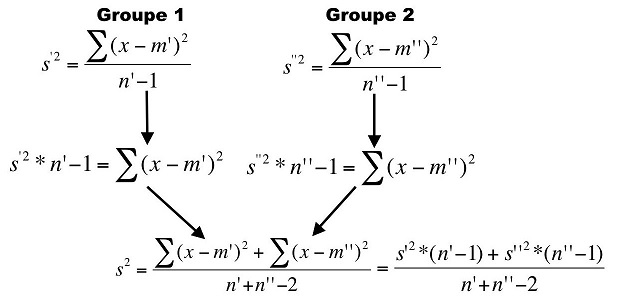
\includegraphics{compositionVariance.jpg}

\emph{Figure 2 Composition des variances corrigées des échantillons pour
estimer la variance parente}

Dans le cas des groupes indépendants, l'estimation de la variance
parente se fait en composant les variances des deux groupes.
Concrètement, le groupe 1 a pour variance \(s’^2\) et le groupe 2,
\(s’’^2\). En multipliant les variances corrigées de chacun des deux
groupes par le nombre d'observations, on obtient les sommes des carrés
des écarts à la moyenne pour chacun des groupes. La variance corrigée de
la réunion des deux groupes peut alors être estimée en additionnant ces
deux sommes des carrés et en les divisant par la somme des observations
dans les deux groupes moins deux. On peut calculer la variance corrigée
de façon plus directe en utilisant la dernière formule. Avec s2 ainsi
calculé, la formule du t de Student devient la suivante pour les groupes
indépendants.

\(t_{obs} = \frac{m{}'-m{}''}{s\sqrt{\frac{1}{n{}'}+\frac{1}{n{}''}}}\)

Voyons à travers un exemple son application. Reprenons pour cela
l'exemple utilisé pour l'application du test du Z, mais en faisant
abstraction de la variance parente. Nous avons, ici, 40 sujets répartis
de façon équilibrée dans deux groupes, qui ont chacun eu à résoudre une
version différente de la tour de Hanoi. On observe que le temps moyen de
résolution est de 5 mn et une variance corrigée de 5,76 pour la version
standard, et de 7 mn pour la version des ascenseurs, avec une variance
corrigée de 6,25. La question à laquelle on cherche à répondre est la
même que précédemment : peut-t-on dire que le problème des ascenseurs
est plus difficile?

Ne connaissant pas la variance parente, pour répondre à cette question,
nous allons situer l'échantillon à l'aide de la distribution du t de
Student. Commençons par calculer la variance corrigée des deux groupes.
Notons, que nous avons dans l'énoncé les variances corrigées, il faut
donc les multiplier par le nombre d'observations moins 1. Si nous avions
eu les variances, c'est par le nombre d'observations qu'il aurait fallu
les multipliées pour retrouver la somme des carrés des écarts.

\(s^{2} = \frac{5,76*(20-1)+6.25*(20-1)}{20+20-2} = 6,005\)

Ce calcul nous permet d'obtenir la variance corrigée correspondant à la
réunion des deux groupes. Il n'y a plus qu'à extraire la racine carré
pour obtenir l'écart-type corrigé.

\(s = \sqrt{6,005} = 2,451\)

Nous pouvons maintenant appliquer la formule du t de Student.

\(t_{obs} = \frac{m{}'-m{}''}{s\sqrt{\frac{1}{n{}'}+\frac{1}{n{}''}}} = \frac{5-7}{2,451\sqrt{\frac{1}{20}+\frac{1}{20}}} = -2,58\)

Dans cet exemple, \(t_{obs}\) est égal à -2,58. Nous allons maintenant
situer cette valeur dans la distribution du t de Student.

Unilatéral

0,3

0,2

0,1

0,05

0,025

0,01

0,005

0,001

Bilatéral

0,6

0,4

0,2

0,1

0,05

0,02

0,01

0,002

ddl

1

0,73

1,38

3,08

6,31

12,71

31,82

63,66

318,31

2

0,62

1,06

1,89

2,92

4,30

6,96

9,92

22,33

3

0,58

0,98

1,64

2,35

3,18

4,54

5,84

10,21

4

0,57

0,94

1,53

2,13

2,78

3,75

4,60

7,17

\ldots{}

\ldots{}

\ldots{}

\ldots{}

\ldots{}

\ldots{}

\ldots{}

\ldots{}

\ldots{}

28

0,53

0,85

1,31

1,70

2,05

2,47

2,76

3,41

29

0,53

0,85

1,31

1,70

2,05

2,46

2,76

3,40

30

0,53

0,85

1,31

1,70

2,04

2,46

2,75

3,39

40

0,53

0,85

1,30

1,68

2,02

2,42

2,70

3,31

\emph{Tableau 16 Lecture dans la table du t de Student}

Dans notre exemple, \(t_{obs}\) égale 2,58. Nous avons 20 observations
donc 38 degrés de liberté. C'est donc la ligne 38 qu'il nous faudrait
regarder. Comme souvent dans les tables disponibles dans les ouvrages de
statistiques, celles-ci, faute de place, ne contiennent pas toutes les
valeurs possibles. Dans ce cas, on se réfère à la ligne la plus proche
inférieure. Vous avez, en effet, pu remarquer que plus on descend dans
la table, moins les valeurs sont importantes. Une approximation par
excès risque donc de nous conduire à déclarer significatif un résultat
qui ne l'est pas. En faisant une approximation par défaut, on est
assuré, si on déclare un résultat significatif, il l'est pour un nombre
de degré de liberté plus important. Nous consulterons donc la table à la
ligne 30.

Nous cherchons ensuite sur cette ligne la valeur inférieur ou égale la
plus proche à notre \(t_{obs}\), en ne considérant que sa valeur
absolue. Cette valeur est de 2,46. Nous testons l'hypothèse que les
sujets mettent moins de temps à résoudre le problème standard que ceux
qui ont résolu le problème des ascenseurs. Notre hypothèse est donc
orientée du coté des valeurs basses. En conséquence, nous regarderons le
seuil unilatéral, et lisons en tête de colonne la proportion recherchée.
Elle est de .010. Cette proportion est inférieure à ce seuil. Notre
table n'étant pas assez précise, cette valeur n'est qu'une approximation
et il serait plus juste de dire que la valeur de p est comprise entre
.010 et .005. En fait, un tableur ou un logiciel de statistique, nous
renverrais une valeur de p égale à .007. La lecture dans la table n'est
donc qu'une approximation, mais celle-ci est suffisante pour faire
l'inférence.

D'un point de vue statistique, l'interprétation du résultat dépend comme
toujours du modèle d'échantillonnage dans lequel on se place. Dans le
cadre du modèle combinatoire, dans lequel on peut toujours se placer, on
teste l'homogénéité des groupes. Autrement dit, on teste l'idée que les
sujets des deux groupes peuvent éventuellement être mélangés. Dans cet
exemple, on peut également se placer d'un point de vue fréquentiste. On
peut en effet considérer que les sujets sont affectés à l'un ou l'autre
des problèmes de façon aléatoire. Toutes choses égales par ailleurs, nos
sujets ne diffèrent donc que par le type de problème qu'ils ont à
résoudre. Dans ce modèle d'échantillonnage, la proportion sera
interprétée comme une probabilité d'obtenir une telle différence de
moyenne dans une distribution d'échantillonnage centrée sur 0. Cette
probabilité est suffisamment faible pour qu'on puisse rejeter
l'hypothèse nulle sans grand risque de se tromper.

D'un point de vue psychologique, la comparaison de deux problèmes
isomorphes, c'est-à-dire ayant la même structure logique, mais pas le
même contenu sémantique, permet d'étudier le rôle des aspects
sémantiques dans la construction de l'interprétation d'un problème. Nous
voyons, dans cet exemple que les deux problèmes ne sont pas équivalents
et que, pour répondre à la question, le problème des ascenseurs est plus
difficile que le problème standard, ce qui montre que la représentation
qu'on s'en fait permet moins facilement d'évoquer des procédures de
résolution pertinentes.

\hypertarget{inference-sur-un-protocole-bivarie}{%
\chapter{INFERENCE SUR UN PROTOCOLE
BIVARIE}\label{inference-sur-un-protocole-bivarie}}

Dans le cas des protocoles bivariés, la distribution exacte est donnée
par l'ensemble des permutations. Celle-ci ayant déjà été présentée
(\textbf{chapitre ???}), nous n'y reviendrons pas.

\hypertarget{inference-sur-un-protocole-bivarie-numerique}{%
\section{Inférence sur un protocole bivarié
numérique}\label{inference-sur-un-protocole-bivarie-numerique}}

Dans le cas de l'étude de la liaison entre deux variables numériques,
nous avons un couple d'observations sur ces deux variables pour chacun
des sujets. Dans ce cas, la distribution exacte est l'ensemble des
permutations possibles. Elle a déjà été développée dans le chapitre sur
les protocoles univarié appariés, c'est pourquoi elle ne sera pas
reprise dans le cadre des protocoles bivariés. D'un certain point de
vue, les données d'un protocole bivarié ressemblent à ce que nous avons
vu dans les structures appariées où nous avons également un couple
d'observations pour chaque sujet. Le questionnement est cependant très
différent. Dans les protocoles univariés structurées, c'est la même
variable dépendante qui est recueillie dans deux conditions. La question
de la comparaison a du sens puisque la différence entre les deux
conditions est testée sur une même dimension. Dans le cas des protocole
bivariés, les séries de données ne correspondent pas à la même
dimension.

\(r = \frac{\sum (x_{i}-m_{x})(y_{i}-m_{y})}{\sqrt{\sum (x_{i}-m_{x})^{2}\sum (y_{i}-m_{y})^{2}}}\)

Dans l'analyse des protocoles bivariés, on cherche à savoir si les
variations sur une variable s'accompagnent ou non de variations sur
l'autre variable. Pour cela, vous avez vu en première année qu'on
calculait le r de Bravais-Pearson qui permet d'évaluer la proximité
entre les données et une liaison linéaire. Dans de cas, l'hypothèse
nulle correspond à un r égal à 0, autrement dit à l'absence de liaison
entre les variables.

\(T = \frac{r\sqrt{n-2}}{\sqrt{1-r^{2}}}\)

Si on dispose d'une table des valeurs critiques de r, on peut lire
directement dans la table, pour n-2 degrés de liberté, la proportion
associée à une valeur critique de \(r\). A défaut de cette table, pour
tester cette hypothèse nulle, on peut utiliser le t de Student en
adaptant la formule (\textbf{Rouanet, 1990}). Cette statistique est
approximativement distribuée comme le t de Student à n-2 degrés de
liberté.

Voyons un exemple de sa mise en oeuvre. Dans l'étude de la résolution de
problèmes comme la tour de Hanoi, il est classique de prendre comme
indicateurs de difficulté le temps et le nombre d'actions réalisées pour
parvenir à la solution. On fait l'hypothèse que ces deux indicateurs
reflètent des processus très différents dans la recherche de solution
par un sujet. En effet, on peut observer chez certains sujets un temps
de résolution long accompagné d'un nombre réduit d'actions, ce qui peut
traduire une importante propension à la réflexion avant l'action. A
l'inverse, certains sujets réalisent une très grand nombre d'actions et
résolvent rapidement le problème, ce qui peut être interpréter comme une
importante propension à l'action. Si ces deux indicateurs reflètent bien
des dimensions différentes et pour ainsi dire antagonistes, de la
difficulté d'un problème, on devrait observer une corrélation négative
entre les deux variables. Les observations recueillies sur un
échantillon de 30 sujets ayant eu à résoudre une variante de la tour de
Hanoi permettent d'observer un \(r\) de -0,57.

Nous ne reviendrons pas sur le calcul du r de Bravais-Pearson dans le
cadre de ce cours. Nous renvoyons les étudiants qui ne se souviendraient
plus de la procédure de calcul de cette statistique à leur cours de
première année. Voyons d'abord la lecture de la table des valeurs
critiques de r.

ddl

0,2

0,1

0,05

0,02

0,01

0,001

0,0001

0,00001

1

0,95

0,99

1

1

1

1

1

1

2

0,8

0,9

0,95

0,98

0,99

1

1

1

3

0,69

0,81

0,88

0,93

0,96

0,99

1

1

\ldots{}

\ldots{}

\ldots{}

\ldots{}

\ldots{}

\ldots{}

\ldots{}

\ldots{}

\ldots{}

27

0,25

0,31

0,37

0,43

0,47

0,58

0,66

0,72

28

0,24

0,31

0,36

0,42

0,46

0,57

0,65

0,71

29

0,24

0,3

0,36

0,42

0,46

0,56

0,64

0,7

30

0,23

0,3

0,35

0,41

0,45

0,55

0,63

0,7

\emph{Tableau 1 Lecture de la table du r}

La lecture de la table se fait à la ligne correspondant à n-2 degrés de
libertés. Dans notre exemple, nous avons n=30 et donc 30-2=28 degrés de
liberté. Avec le r de Bravais Pearson, la force de la liason est donnée
par la valeur absolue de r et la direction de la liaison par le signe de
r. Ici, nous cherchons à faire une inférence sur la force de la liaison.
Les valeurs dans la table sont donc des valeurs absolues. Comme à chaque
fois avec ce type de table, nous cherchons la valeur inférieure ou égale
à la valeur observée. Nous trouvons 0,57. Il suffit alors de lire en
tête de colonne la proportion associée. Cette procédure, très simple,
masque les aspects conceptuels de l'inférence sur ce type de protocole.
On situe en fait notre échantillon dans une distribution des coéfficient
de Bravais-Pearson centrée sur 0. Cette distribution peut également être
approchée à l'aide de la distribution de t de Student. Il faut pour cela
adapter la formule comme suit :

\(t = \frac{r\sqrt{n-2}}{\sqrt{1-r^{2}}} = \frac{-0,57\sqrt{30-2}}{\sqrt{1-(-0,57)^{2}}} = 3,67\)

Dans notre exemple, \(t_{obs}\) est égal à 3,67. Nous allons maintenant
situer cette valeur dans la distribution du \(t\) de Student. Nous avons
30-2=28 ddl. C'est donc la ligne 28 qu'il nous faut regarder. On y
recherche la valeur la plus proche et inférieure ou égale à tobs. Ici
tobs=3,67. La valeur la plus proche dans la table est 3,41. Dans notre
exemple, l'hypothèse est orientée du côté des valeurs basses. C'est donc
à un seuil unilatéral qu'il faut consulter la table. La proportion
recherchée est donc de .001. Cette proportion étant inférieure au seuil
repère de .025, le résultat peut être déclaré significatif.

Comme à chaque fois, l'interprétation du test dépend du modèle
d'échantillonnage dans lequel on se place. Dans le modèle combinatoire,
on teste la typicité de l'échantillon dans une distribution de r centrée
sur 0, donc dans une distribution où il n'y a pas de relation linéaire
entre les deux variables. Dans notre exemple, le fait de trouver un
résultat significatif nous permet de conclure à l'atypicité de
l'échantillon dans une telle distribution.

On peut également se placer dans le modèle fréquentiste. Dans le cadre
de ce modèle, on teste l'hypothèse d'un coefficient de corrélation nul
dans la population parente. La proportion est alors interprétée comme
une probabilité d'obtenir un échantillon comme celui qu'on a observé
dans la population parente. On voit qu'ici, cette proportion est
suffisamment faible pour qu'on puisse accepter de rejeter l'hypothèse
nulle, avec un risque de 1 pour 1000 de se tromper. On peut donc
conclure à l'existence d'une relation linéaire, ce qui d'un point de vue
psychologique étaye l'hypothèse que ces deux indicateurs reflètent des
dimensions différentes de la difficulté d'un problème.

\hypertarget{inference-sur-un-protocole-bivarie-nominal}{%
\section{Inférence sur un protocole bivarié
nominal}\label{inference-sur-un-protocole-bivarie-nominal}}

\hypertarget{cas-des-variables-dichotomiques}{%
\subsection{Cas des variables
dichotomiques}\label{cas-des-variables-dichotomiques}}

Dans le cas de l'inférence sur un protocole bivarié, la distribution
exacte est également la distribution hypergéométrique pour les tableaux
de contingence à quatre cases. Il s'agit d'évaluer la liaison entre deux
variables c'est-à-dire chercher si certaines modalités d'une des
variables sont associées préférentiellement à certaines modalités de
l'autre variables ou si au contraire elles ont tendance à s'exclure. Ce
test est formellement équivalent au test sur la fréquence dans le cas
des tableaux à 4 cases. En voici un petit exemple.

Le directeur d'une usine d'assemblage d'automobiles s'interroge sur la
pénibilité du travail des ouvriers sur la chaîne de montage des
carrosseries. Il prend pour critère le nombre d'arrêts de travail suite
à l'apparition de troubles musculo-squelettiques (TMS) chez les
ouvriers. Suite à une première enquête, il semblerait que les ouvriers
de plus de 45 ans soient davantage exposés aux TMS que les autres
ouvriers de la chaîne. Un ergonome est chargé de réaliser une étude plus
approfondie sur la question. Les données observées sont les suivantes :

Arrêts

Pas d'arrêt

Total

\textgreater{}45 ans

9

6

15

≥ 45 ans

7

18

25

Total

16

24

40

\emph{Tableau 2 Répartition des ouvriers en fonction de l'âge et de la
survenue de TMS}

Parmi les 15 ouvriers de plus de 45 ans, 9 ont eu un arrêt de travail
dans les 6 derniers mois en raison de TMS, ce qui représente une
fréquence de près des deux tiers. Cela suffit-il à dire que les ouvriers
de plus de 45 ans sont plus sujets que les autres aux TMS ? Pour
répondre à cette question, il faut chercher dans la distribution
d'échantillonnage la proportion d'échantillons présentant une fréquence
d'arrêts de travail supérieure ou égale à 9/15. Cette proportion nous ai
donnée par la distribution hypergéométrique, avec les valeurs de \(k\)
allant de 9 à 15.

\(k\)

\(n-k\)

\(A-k\)

\(N-A-(n-k)\)

\(p_{k}\)

\(p_{k}\) cumulé

9

3

7

18

0,03827881

0,03827881

10

4

6

19

0,00846163

0,04674044

11

5

5

20

0,00115386

0,04789430

12

6

4

21

0,00009158

0,04798588

13

7

3

22

0,00000384

0,04798972

14

8

2

23

0,00000007

0,04798979

15

9

1

24

0

0,04798979

\emph{Tableau 3 Distribution hypergéométrique sur l'exemple des TMS chez
les ouvriers}

La proportion cumulée est de .05. Elle supérieure au seuil-repère .025.
En conséquence, le résultat est non significatif. On ne peut donc pas
dire que les arrêts de travail pour cause de TMS soient plus fréquents
chez les ouvriers de plus de 45 ans dans cette usine. Comme pour tous
les protocoles nominaux, la distribution d'échantillonnage peut être
approchée avec la distribution de \(\chi^{2}\) à 1 ddl. Mais il faut
appliquer la correction de continuité et veiller à ce qu'aucun effectif
théorique ne soit inférieur à 5.

Effectifs observés

Arrêts

Pas d'arrêt

Total

\textgreater{}45 ans

9

6

15,00

≥ 45 ans

7

18

25,00

Total

16,00

24,00

40,00

Effectifs théoriques

Arrêts

Pas d'arrêt

Total

\textgreater{}45 ans

6

9

15,00

≥ 45 ans

10

15

25,00

Total

16,00

24,00

40,00

Contributions à \(\chi^{2}\)

Arrêts

Pas d'arrêt

Total

\textgreater{}45 ans

1,04

1,36

2,40

≥ 45 ans

1,23

0,42

1,64

Total

2,27

1,78

4,04

\emph{Tableau 4 Calcul de \(\chi ^{2}\) sur l'exemple des TMS chez les
ouvriers}

Dans cet exemple, nous avons donc :

\(\chi ^{2}_{corr} = \frac{\left ( \left | 9-6 \right | -0,5 \right )^{2}}{6}+\frac{\left ( \left | 6-9 \right | -0,5 \right )^{2}}{9} + \frac{\left ( \left | 7-10 \right | -0,5 \right )^{2}}{10} +\frac{\left ( \left | 18-15 \right | -0,5 \right )^{2}}{15} = 2,78\)

Nous avons dans ce cas un degré de liberté. La lecture de la table se
fera sur la première ligne. La valeur la plus proche inférieure à la
valeur calculée est, dans cette table, 2,71. Elle correspond à une
proportion de .10. Cette table fournie des proportions bilatérales, il
est donc normale de trouver une proportion du double de celle trouvée
avec la distribution exacte qui était une proportion unilatérale. La
conclusion sera donc la même que précédemment.

\hypertarget{cas-des-variables-a-plus-de-deux-modalites.}{%
\subsection{Cas des variables à plus de deux
modalités.}\label{cas-des-variables-a-plus-de-deux-modalites.}}

Pour décrire cette liaison, vous avez vu en première année qu'on utilise
le coefficient de contingence phi-deux. Cette statistique étant le
rapport de khi-deux sur n, on peut tout naturellement utiliser la
distribution de khi-deux pour faire l'inférence. L'hypothèse testée est
alors celle d'une équirépartition des observations sur les différentes
modalités du croisement des variables, autrement dit le tableau des
effectifs théoriques. On dit qu'on teste l'indépendance entre les
variables.

Voyons à l'aide d'un exemple comment mettre en œuvre le test. Imaginons
qu'on fasse passer à un ensemble d'étudiants un questionnaire sur
l'intérêt des statistiques dans les cours de psychologie. Cet intérêt
est évalué par une question ouverte où on demande aux sujets d'indiquer,
selon eux à quoi servent les statistiques pour un psychologue. On relève
par ailleurs le type de bac que les étudiants ont obtenu. On fait
l'hypothèse que le type de réponse est lié au type de bac des étudiants.

Trois catégories ont été distinguées: les bacs scientifiques, les bacs
littéraires et les bacs technologiques. Les réponses des sujets ont été
regroupées en 4 catégories: ceux qui pensent que les statistiques sont
inutiles, ceux qui pensent qu'elles servent à comprendre ou à faire de
la recherche et enfin ceux qui la vivent comme un moyen de sélection.

Effectifs observés

Inutile

Comprendre la recherche

Faire de la recherche

Moyen de sélection

Total

Scientifique

3

24

16

8

51

Littéraire

7

17

20

15

59

Technologique

9

14

11

18

52

Total

19

55

47

41

162

Effectifs théoriques

Inutile

Comprendre la recherche

Faire de la recherche

Moyen de sélection

Total

Scientifique

5,98

17,31

14,80

12,91

51

Littéraire

6,92

20,03

17,12

14,93

59

Technologique

6,10

17,65

15,09

13,16

52

Total

19

55

47

41

162

Contributions au \(\chi^{2}\)

Inutile

Comprendre la recherche

Faire de la recherche

Moyen de sélection

Total

Scientifique

1,49

2,58

0,10

1,87

6,03

Littéraire

0,00

0,46

0,49

0,00

0,95

Technologique

1,38

0,76

1,11

1,78

5,02

Total

2,87

3,80

1,69

3,65

12,00

\emph{Tableau 5 Calcul de} \(\chi ^{2}\)

Nous ne détaillerons pas la procédure du calcul du \(\chi ^{2}\). Elle a
déjà été présentée dans votre cours de première année. La formule de
calcul est la même que précédemment. La correction de continuité n'est
pas nécessaire, puisque nous avons plus d'un degré de liberté. Le nombre
de degrés de liberté étant en effet le nombre de lignes moins un
multiplié par le nombre de colonne, nous avons dans cet exemple 2*3=6
ddl. A partir des marges du tableau des effectifs observés, nous pouvons
calculer les effectifs théoriques. Aucun de ces effectifs n'étant
inférieur à 5. nous pouvons utiliser la distribution de \(\chi ^{2}\).
Ce dernier tableau présente le résultat des calculs de la statistique.
D'un point de vue descriptif, il est intéressant de regarder les sur
représentations. Nous les signalons en rouge dans le tableau de
\(\chi ^{2}\). On peut voir que les bacheliers scientifiques et
littéraires évoquent plutôt comprendre ou faire de la recherche comme
motivation de l'étude des statistiques en psychologie, tandis que les
bacheliers technologiques les considère plutôt comme inutiles ou les
vivent comme un moyen de sélection. Dans notre exemple, \(\chi ^{2}\)
est égal à 12. Nous avons donc un coefficient  de .006. ce qui dénote
une relation très faible entre les deux variables.

La lecture de la table se fera sur la ligne 6, puisque nous avons 6 ddl.
On y trouve la valeur de 12.59, bien que plus proche dépasse la valeur
observée. Nous nous arrêterons sur 1.64 et nous lirons en tête de
colonne la proportion. Celle-ci est de .10 et elle est supérieure au
seuil repère de .05. Le résultat est donc non significatif. Comme à
chaque fois, l'interprétation du test dépend du modèle d'échantillonnage
dans lequel on se situe. Dans le cadre de l'inférence combinatoire, nous
testons l'hypothèse d'indépendance entre les variables. Dans notre
exemple, le test est non significatif, on conclura donc à l'indépendance
entre les variables, Autrement dit, il n'y a pas de liaison entre les
variables. Si on considère que les sujets sont tirés au hasard dans la
population d'étudiants de psychologie, on peut se placer dans le modèle
fréquentiste. Dans ce cas, l'hypothèse nulle est celle de l'indépendance
entre les variables et la proportion peut être interprétée comme une
probabilité d'obtenir un tel échantillon dans une population où les
variables ne sont pas liées. Les résultats du test n'étant pas
significatif, on ne peut rejeter l'hypothèse nulle.

D'un point de vue psychologique, on conclura que l'opinion sur l'utilité
des statistiques dans les études de psychologie ne dépend pas du type de
baccalauréat détenu par les étudiants.

\bibliography{book.bib,packages.bib}


\end{document}
